%!TEX root = ../thesis.tex
\chapter{Coregistration of High Resolution Rat Histology} % (fold)
\label{cha:coregistration_of_high_resolution_rat_histology}
% If you like chapter abstracts ...
\dblspace
\begin{quote}{\em %!TEX root = ../thesis.tex
The automated registration of hundreds of histological slices to a set of references requires a great measure of experimentation, parameterisation and tuning. This chapter contributes the tools and methods to reconstruct sub-cellular resolution whole-organ histological volumes, based on coherent block face images and accurately faithful to the true geometry of the organ.

We develop an incremental pipeline for the particular application of an entire rat heart volume. We list a range of appropriate preprocessing steps and evaluate two methods of transform initialisation. We discuss which metrics and optimisation strategies prove most successful in this context. We outline the most important architectural patterns which lead to code quality and maintainability, and which facilitate rapid prototyping and feedback with limited and diverse computational resources. We develop diagnostic tools to gain deep quantitative insight into the evolution of the registration algorithm, and with the indispensible information gleaned from them, we illustrate a solid general approach to parameter tuning. We showcase the registered rat heart volume, to serve as an anatomical reference, to validate current anatomical models used in simulation, and to inform future experimental and computational technique.
}\end{quote}

\section{Aims} % (fold)
\label{sec:aims}

  Having shown in an idealised geometry that fibre direction could have a significant effect on propagation, the challenge is set to characterise cardiac tissue at sufficient detail to resolve both fibre direction and other microstructure. Cell type distribution, the shape of tissue boundaries, the Purkinje fibre network, sheet structure and vasculature all affect macroscopic wave propagation, and must therefore be incorporated into electrophysiological models.
	
  The aim of this chapter is to develop an automated pipeline to register high resolution rat cardiac datasets robustly and accurately, and generate for the first time coherent whole-organ subcellular resolution 3D cardiac histological images. One full rat heart dataset will be processed through the pipeline to provide registered volumes. These images will serve both as an authoritative anatomical reference, and as the basis for anatomically based models in simulation studies, laying the foundations for the investigation of the role of microstructure in propagation dynamics.
	
% section aims (end

\section{Methods} % (fold)
\label{sec:methods}
	The methods developed to fulfil the aims of this work form the meat of the chapter. First we discuss the experimental acquisition, curation and digital preparation of the images. We go on to cover the algorithms that calculate reasonable starting transformations and refine those transformations via iterative registration. An overview of the tools' architecture precedes the methods developed for diagnostics and parameter tuning.
	
  \subsection{Image Acquisition} % (fold)
  \label{sub:image_acquisition}
    Hearts were isolated from female rats and cannulated via the aorta to a Langendorff perfusion system, in a similar manner to that presented in \cite{Burton2006}. The hearts were then fixed and stabilised in agar, and 25.4 x 25.4 x 12.7$\mu$m MRI scans were performed. The hearts were immersed in increasing concentrations of alcohol, in order to dehydrate them before embedding them in black wax. The wax blocks were then serially sectioned at 10$\mu$m thickness using a microtome. An image of the top surface of the block was taken with 25$\mu$m resolution after each slicing. Every 5th section was Trichrome stained, labelling connective tissue bluish-green, myocytes pinkish-red and nuclei blue-black. Each slice was relaxed and re-hydrated, before histology imaging was performed using a 5x objective with 1.1$\mu$m resolution. Examples of the block face and slice images is displayed in Figures~\labelcref{fig:original_lores_images,fig:original_hires_images}, respectively.
		
		\begin{figure}[htbp]
		  \centering
		  \subfigure[][]{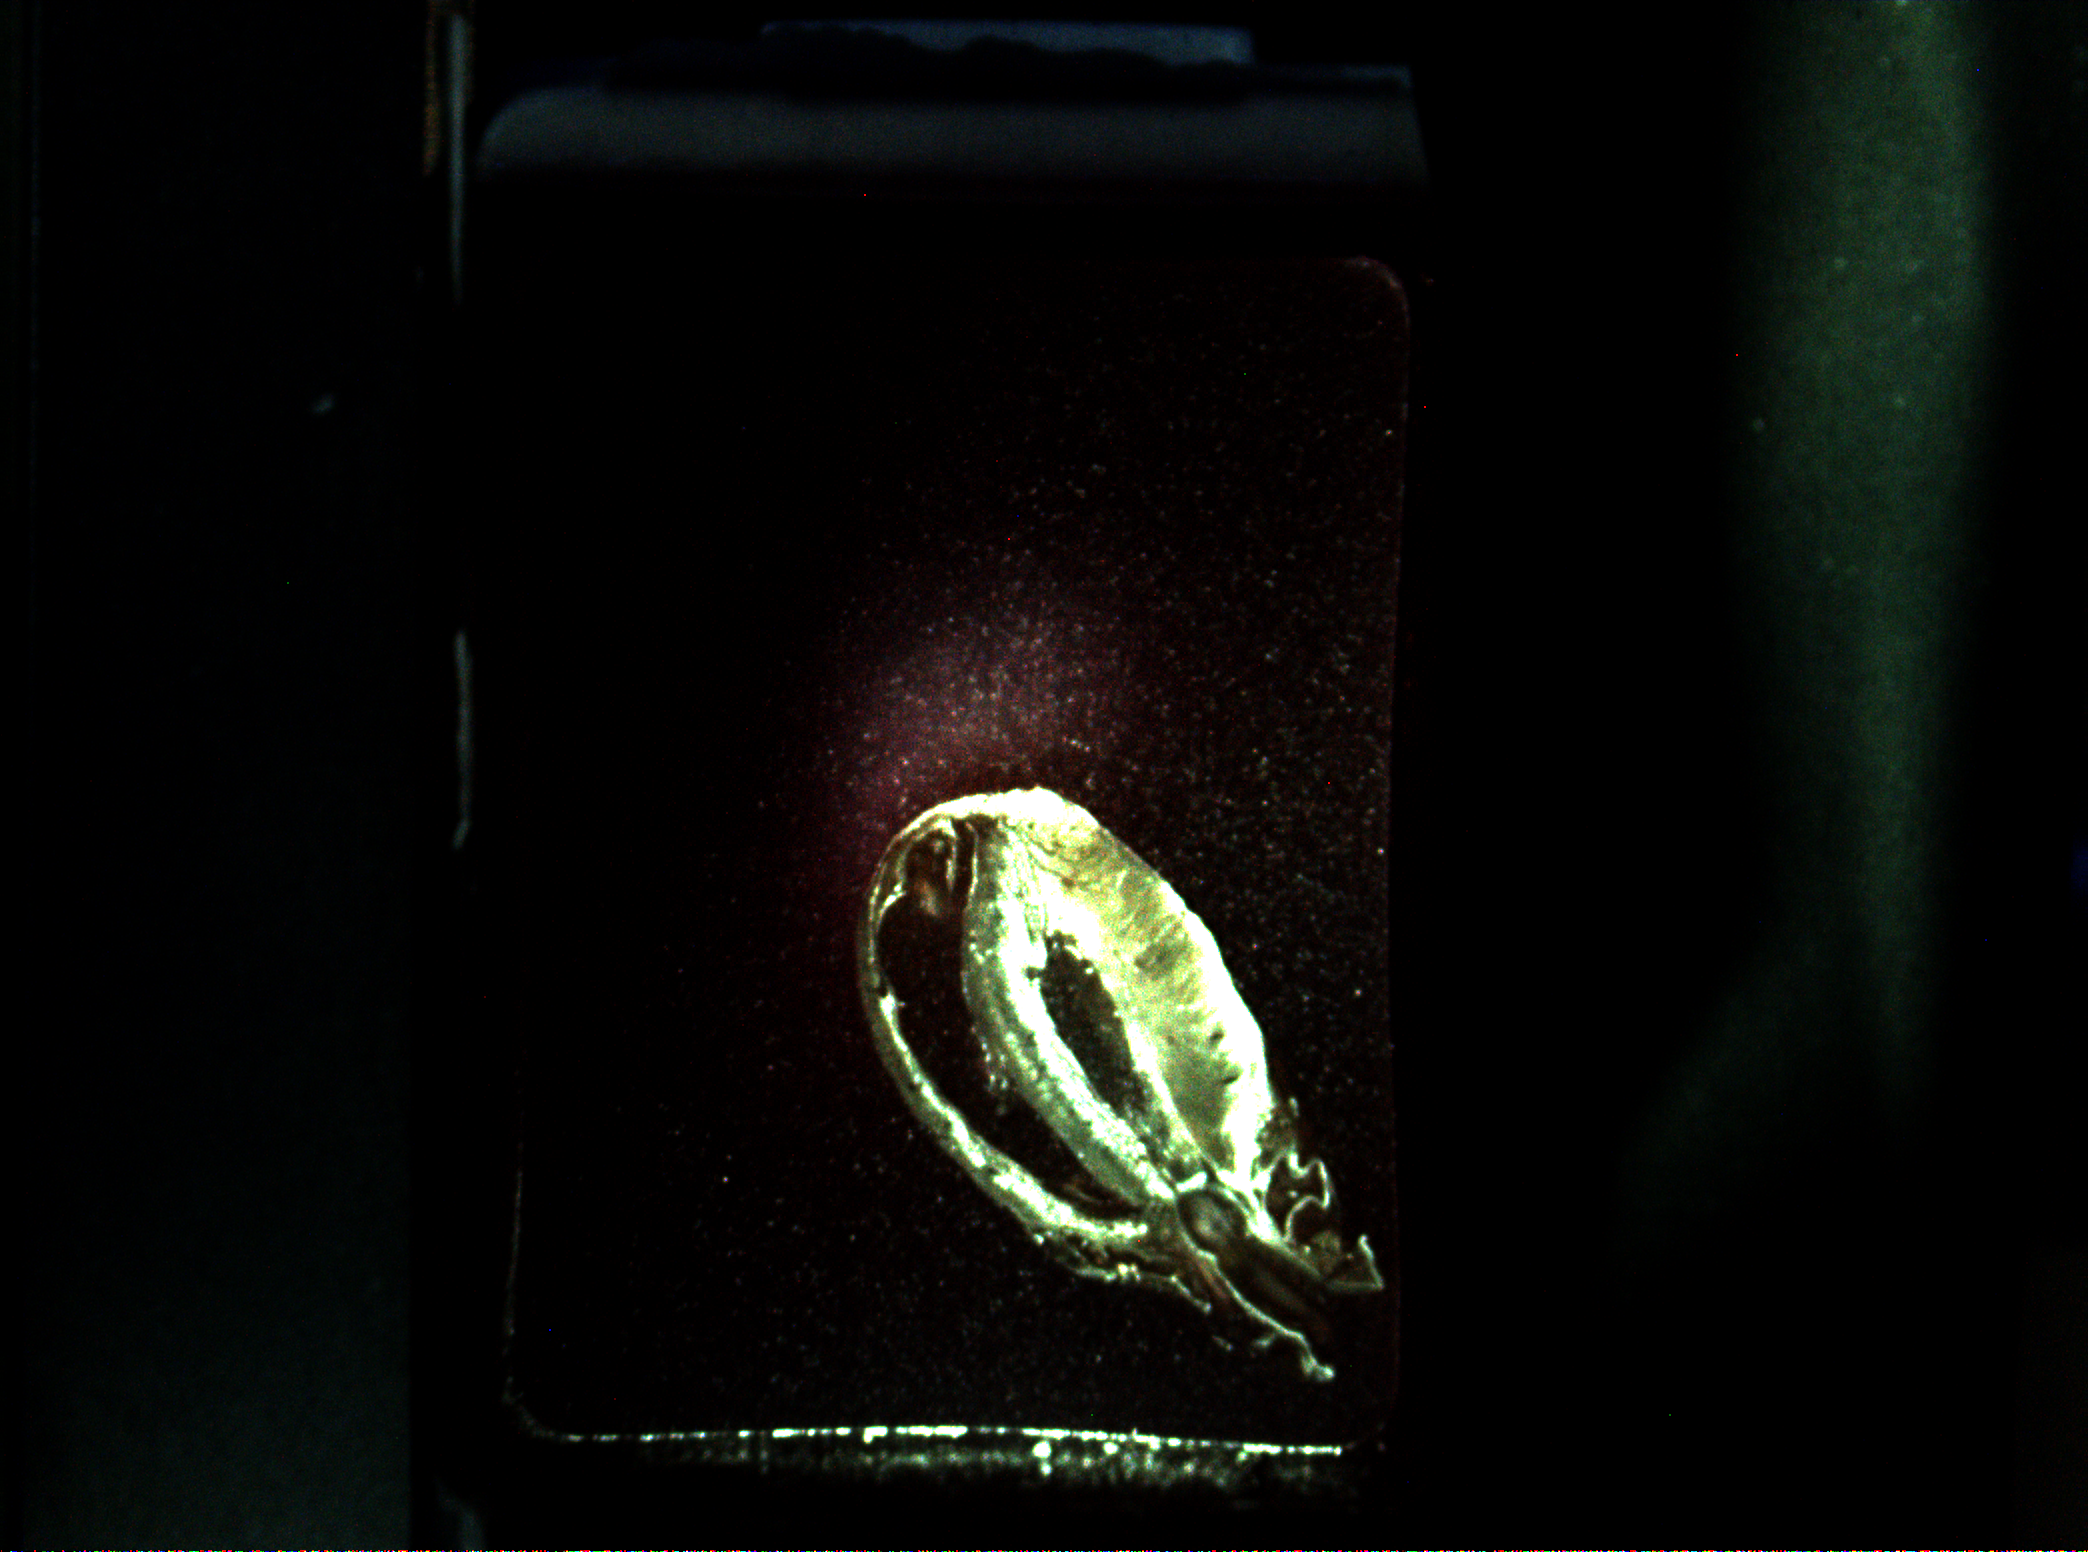
\includegraphics[width=0.8\pagewidth]{Ch5/Figs/LoRes_rgb_downsamples_1_0582}}
		  \subfigure[][]{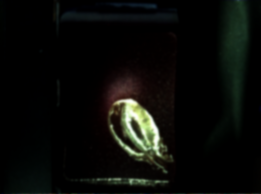
\includegraphics[width=0.8\pagewidth]{Ch5/Figs/LoRes_rgb_downsamples_8_0582}}
		  \caption{Block face images of slice 582 of Rat 28. The original image is shown in \textbf{(a)}, with \textbf{(b)} Gaussian smoothed and downsampled by a factor of 8 in each dimension.}
		  \label{fig:original_lores_images}
		\end{figure}
    
    \begin{figure}[htbp]
      \centering
      \subfigure[][]{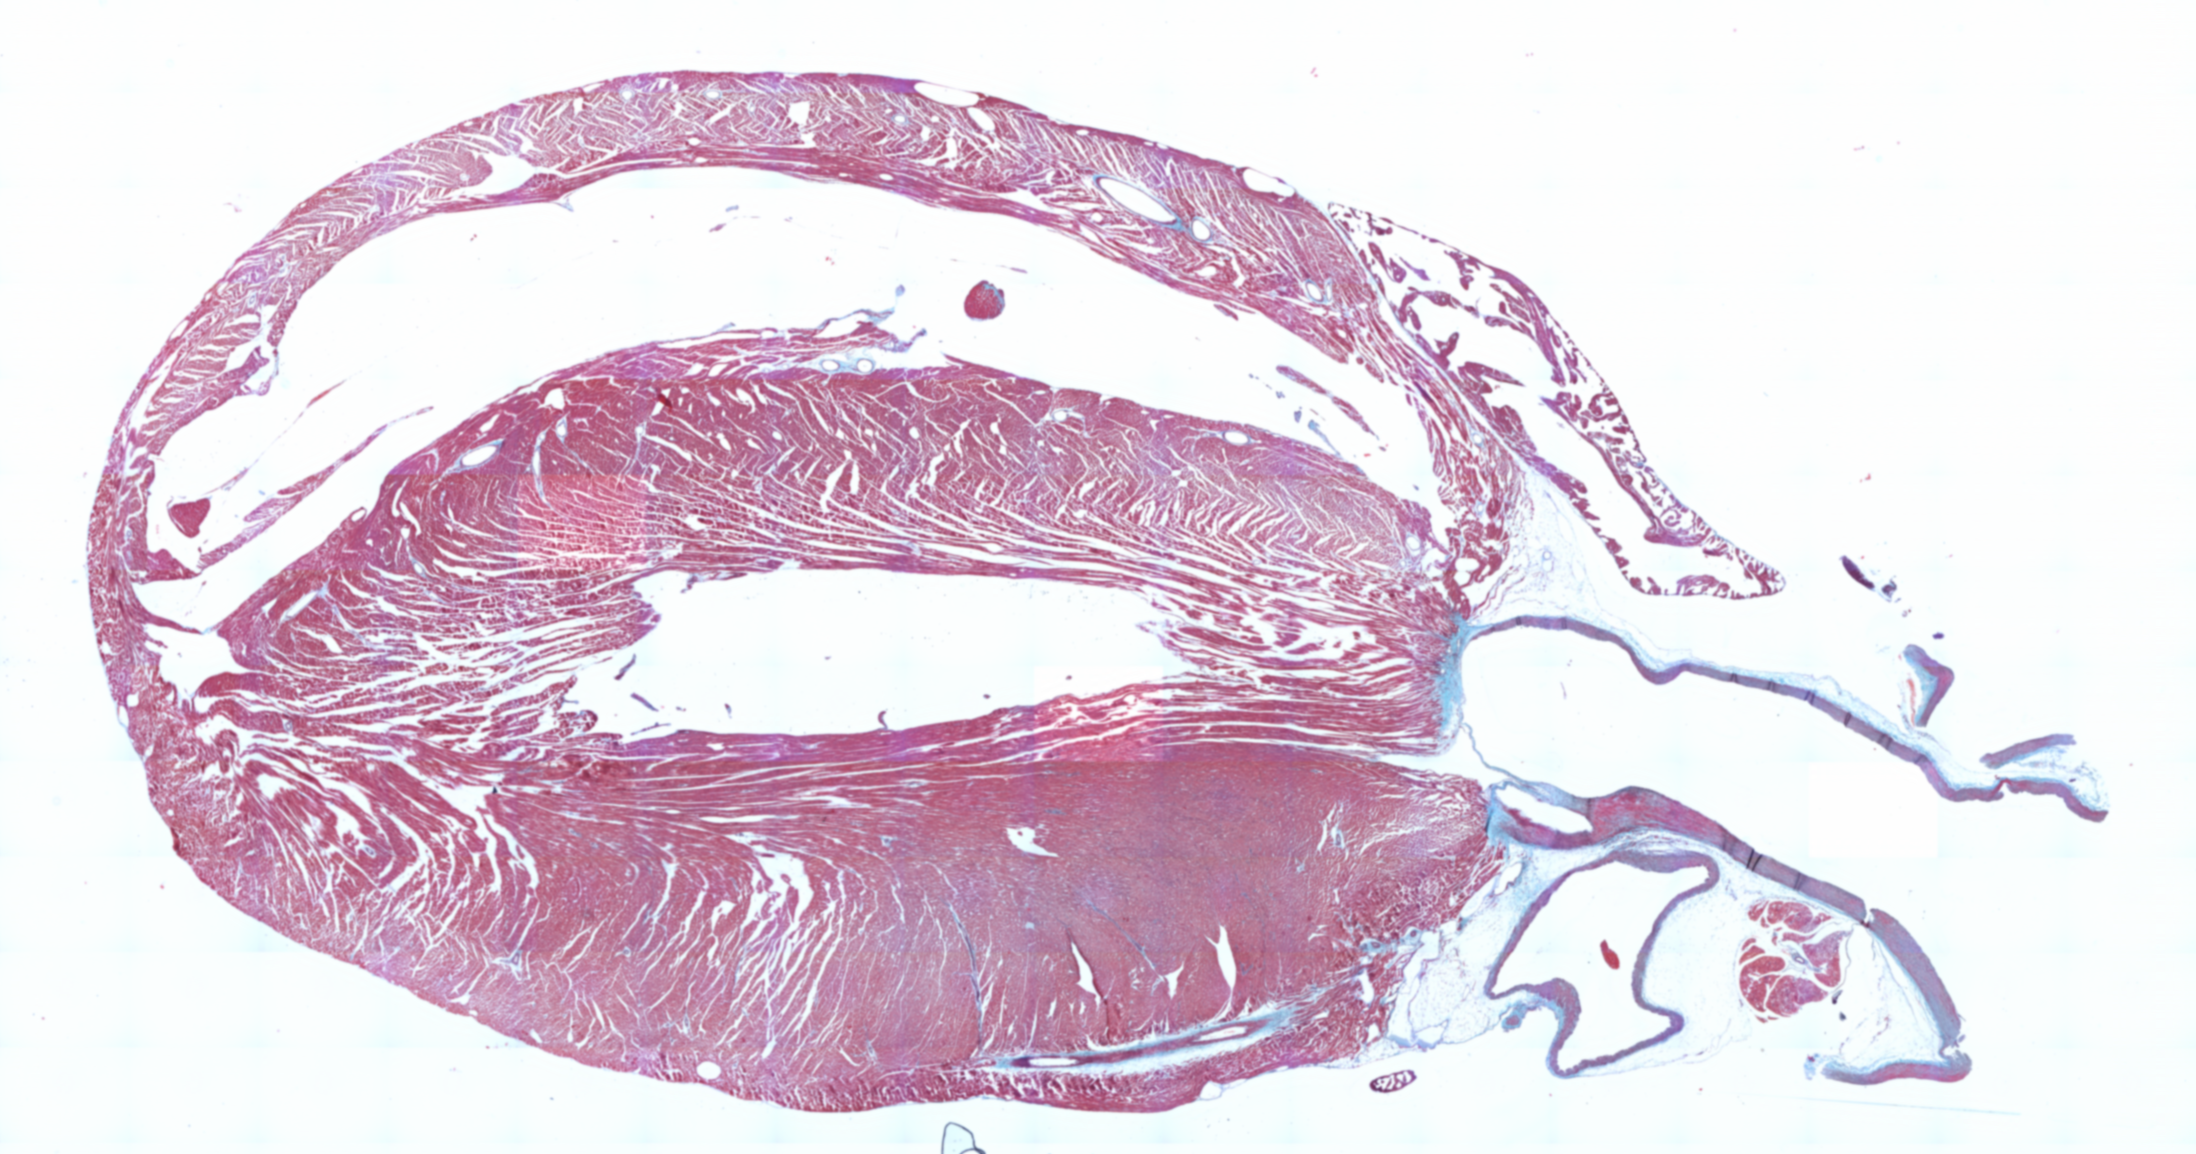
\includegraphics[width=0.8\pagewidth]{Ch5/Figs/HiRes_downsamples_8_0582}}
      \subfigure[][]{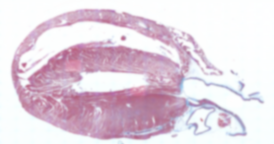
\includegraphics[width=0.8\pagewidth]{Ch5/Figs/HiRes_downsamples_64_0582}}
      \caption{Slice images of slice 582. \textbf{(a)} is Gaussian smoothed and downsampled by a factor of 8, and \textbf{(b)} by 64. The slice must be reflected and rotated in order to align with the block face image in Figure~\ref{fig:original_lores_images}.}
      \label{fig:original_hires_images}
    \end{figure}
	
  % subsection image_acquisition (end)

  \subsection{Image Curation} % (fold)
  \label{sub:image_curation}
    The images provided by Burton et al. yield unprecedented detail and quality. Although every possible step was taken during image acquisition, certain unavoidable experimental practicalities arose. A master subset of the images was selected, removing any slices with unacceptable damage such as that found in Figure~\ref{fig:damaged_slice}. Wherever a slice or group of slices was missing or removed, the acceptable adjacent slices were repeated symmetrically to fill the gap, in order to preserve the macroscopic geometry of the tissue. In the rare case where two images of the same slice existed, both slices were examined and the higher quality version was selected.
    
    \begin{figure}[htbp]
      \centering
      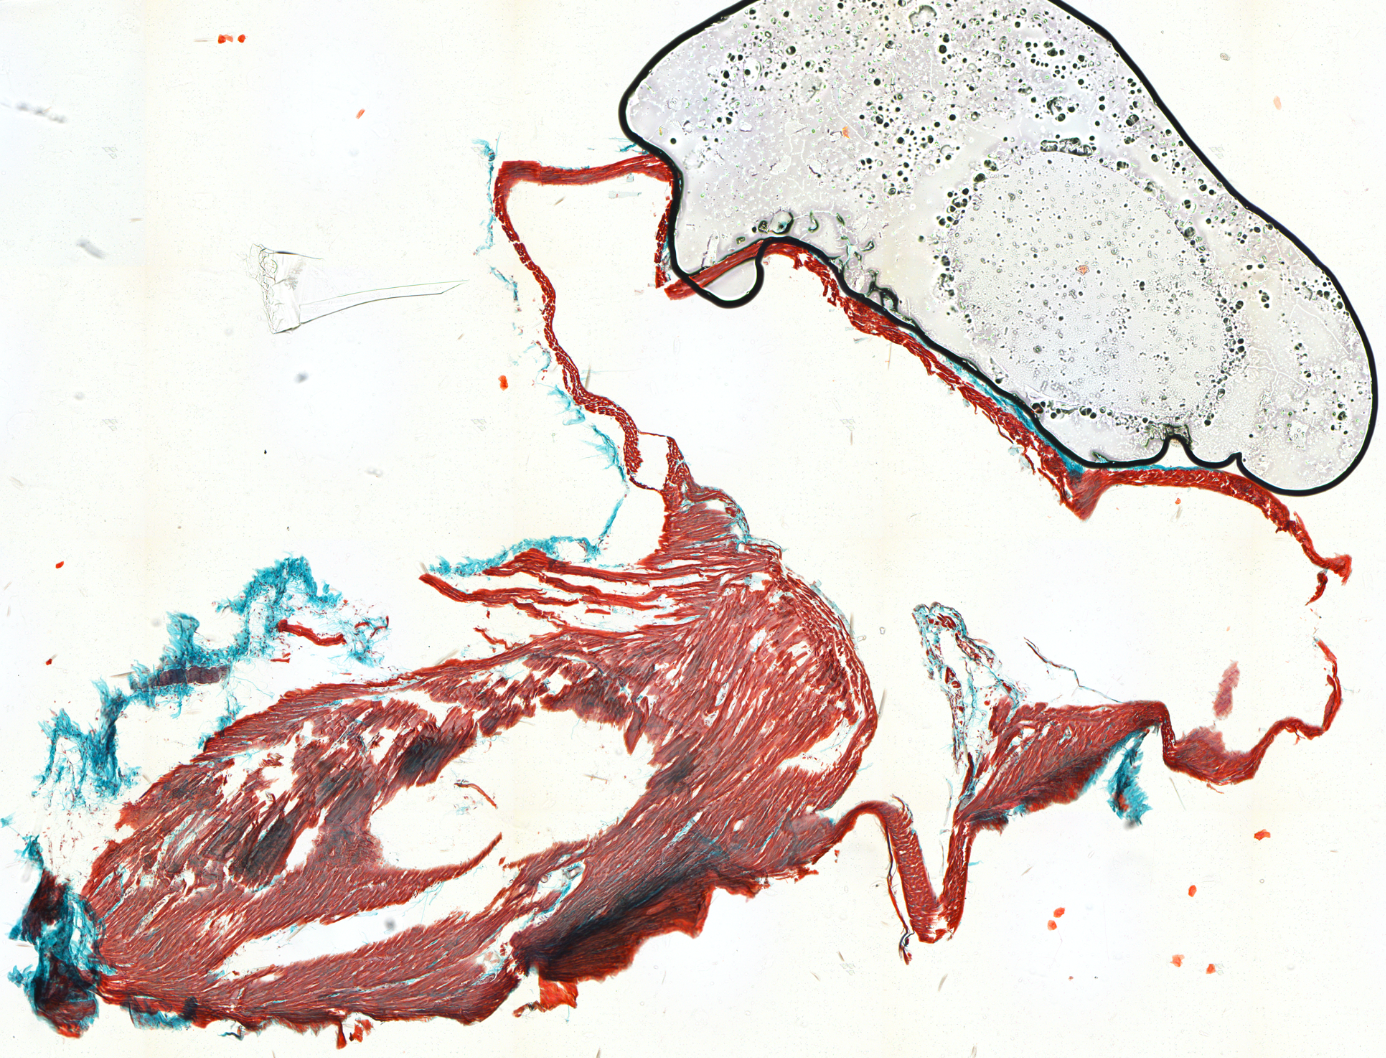
\includegraphics[width=.8\textwidth]{Ch5/Figs/damaged_slice}
      \caption{A damaged slice close to the left extremity of the heart. The tissue is severely damaged and folded in place. There is also a large bubble trapped between the two imaging slides.}
      \label{fig:damaged_slice}
    \end{figure}
    
  % subsection image_curation (end)
  
  \subsection{Image Preparation} % (fold)
  \label{sub:image_preparation}
  	The digital camera used to obtain the images created files with four channels: red, green, blue and alpha. Since transparency is meaningless in the context of a photograph, the fourth alpha channel was uniformly black. Unfortunately, the implementation of the RGBA BMP reader in ITK labels the channels incorrectly, so that the black alpha channel is interpreted as red, the red as green, the green as blue, and the blue as alpha. To correct for this, channels were explicitly permuted and the redundant alpha channel removed.
    
    On occasion, part way through image acquisition, the block face camera would be moved relative to the surface of the wax block. All images acquired from then on had to be translated and rotated to compensate for this movement. At each perturbation, the two slices between which the camera had moved were registered in order to calculate the corrective transform, which was then applied to all subsequent slices. In each case, the parameters from \ref{tab:block_face_to_block_face} were used to optimise a centred rigid transform. Figure~\ref{fig:LoRes_cross_sections} depicts the results of these corrections, and the isosurface of the corrected segmented volume are shown from 6 sides in Figures~\labelcref{fig:LoRes_positive_x,fig:LoRes_negative_x,fig:LoRes_positive_y,fig:LoRes_negative_y,fig:LoRes_positive_z,fig:LoRes_negative_z}. The isosurface was generated from a threshold segmentation of the intensity magnitude of the volume. A dense cloud of wax bubbles and other small artefacts obscured the main surface of the heart, and so a binary shape opening filter was applied to remove all but the largest connected region from the segmentation before the contour was extracted.
    
    % lores cross sections
    \begin{sidewaysfigure}[htbp]
      \centering
      \subfigure[][]{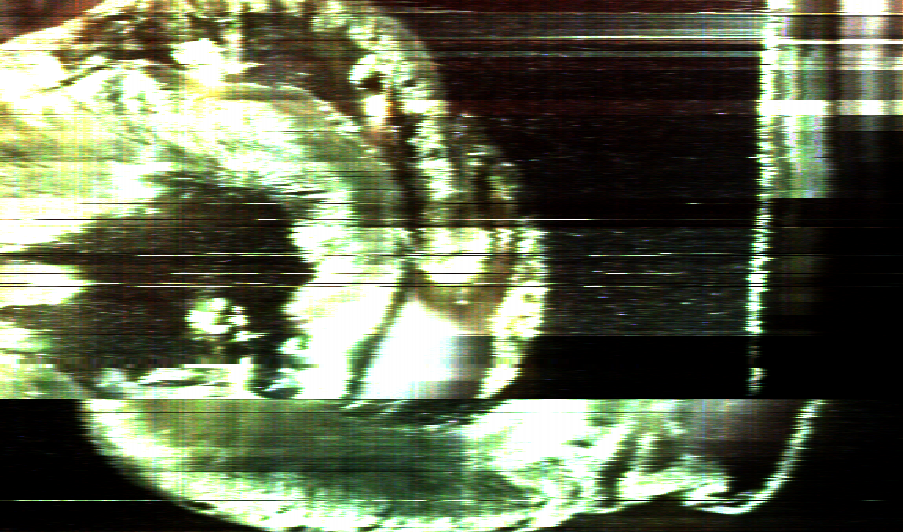
\includegraphics[height=0.31\textheight]{Ch5/Figs/LoRes_without_adjustments_0_235}}
      \subfigure[][]{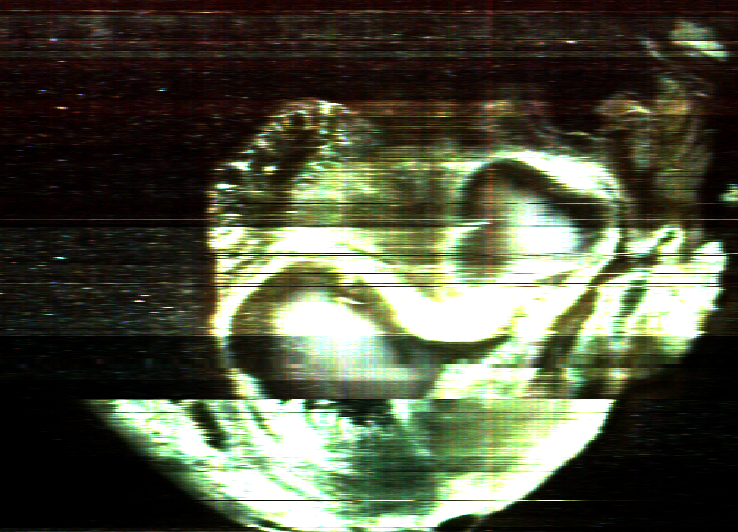
\includegraphics[height=0.31\textheight]{Ch5/Figs/LoRes_without_adjustments_1_287}}
      \subfigure[][]{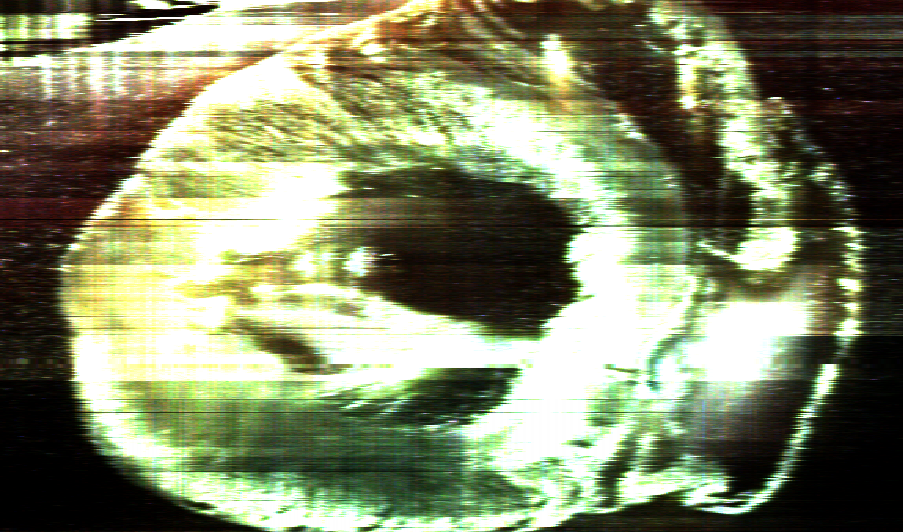
\includegraphics[height=0.31\textheight]{Ch5/Figs/LoRes_0_235}\label{subfig:LoRes_adjusted_long_cross_section}}
      \subfigure[][]{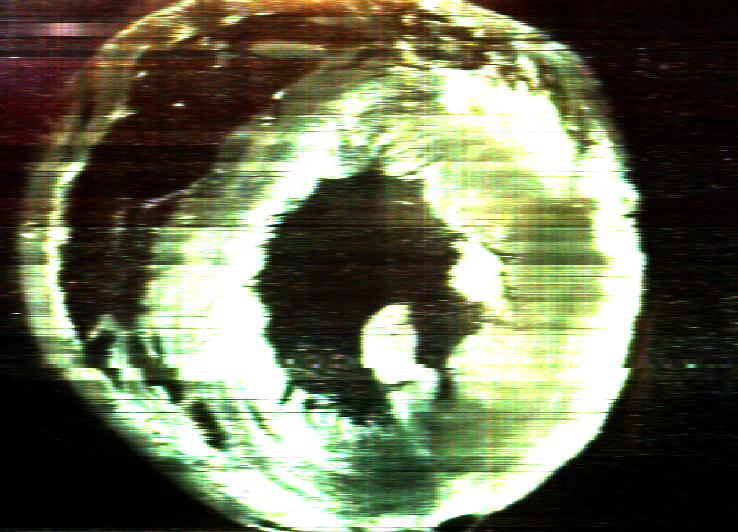
\includegraphics[height=0.31\textheight]{Ch5/Figs/LoRes_1_287}}
      \caption{Central cross-sections of the cropped block-face volume. \textbf{(a)} and \textbf{(b)} show the volume before adjustment, where a large camera displacement is apparent approximately a quarter of the way from the bottom of the image. Several thin stripes are visible further up, where the occasional single image has been displaced. The volume is fully aligned in \textbf{(c)} and \textbf{(d)}, with striations visible due to discrete changes in the positioning and intensity of illumination. These changes will propagate to the final registration result.}
      \label{fig:LoRes_cross_sections}
    \end{sidewaysfigure}
    
    % lores contours
    \begin{sidewaysfigure}[htbp]
      \centering
      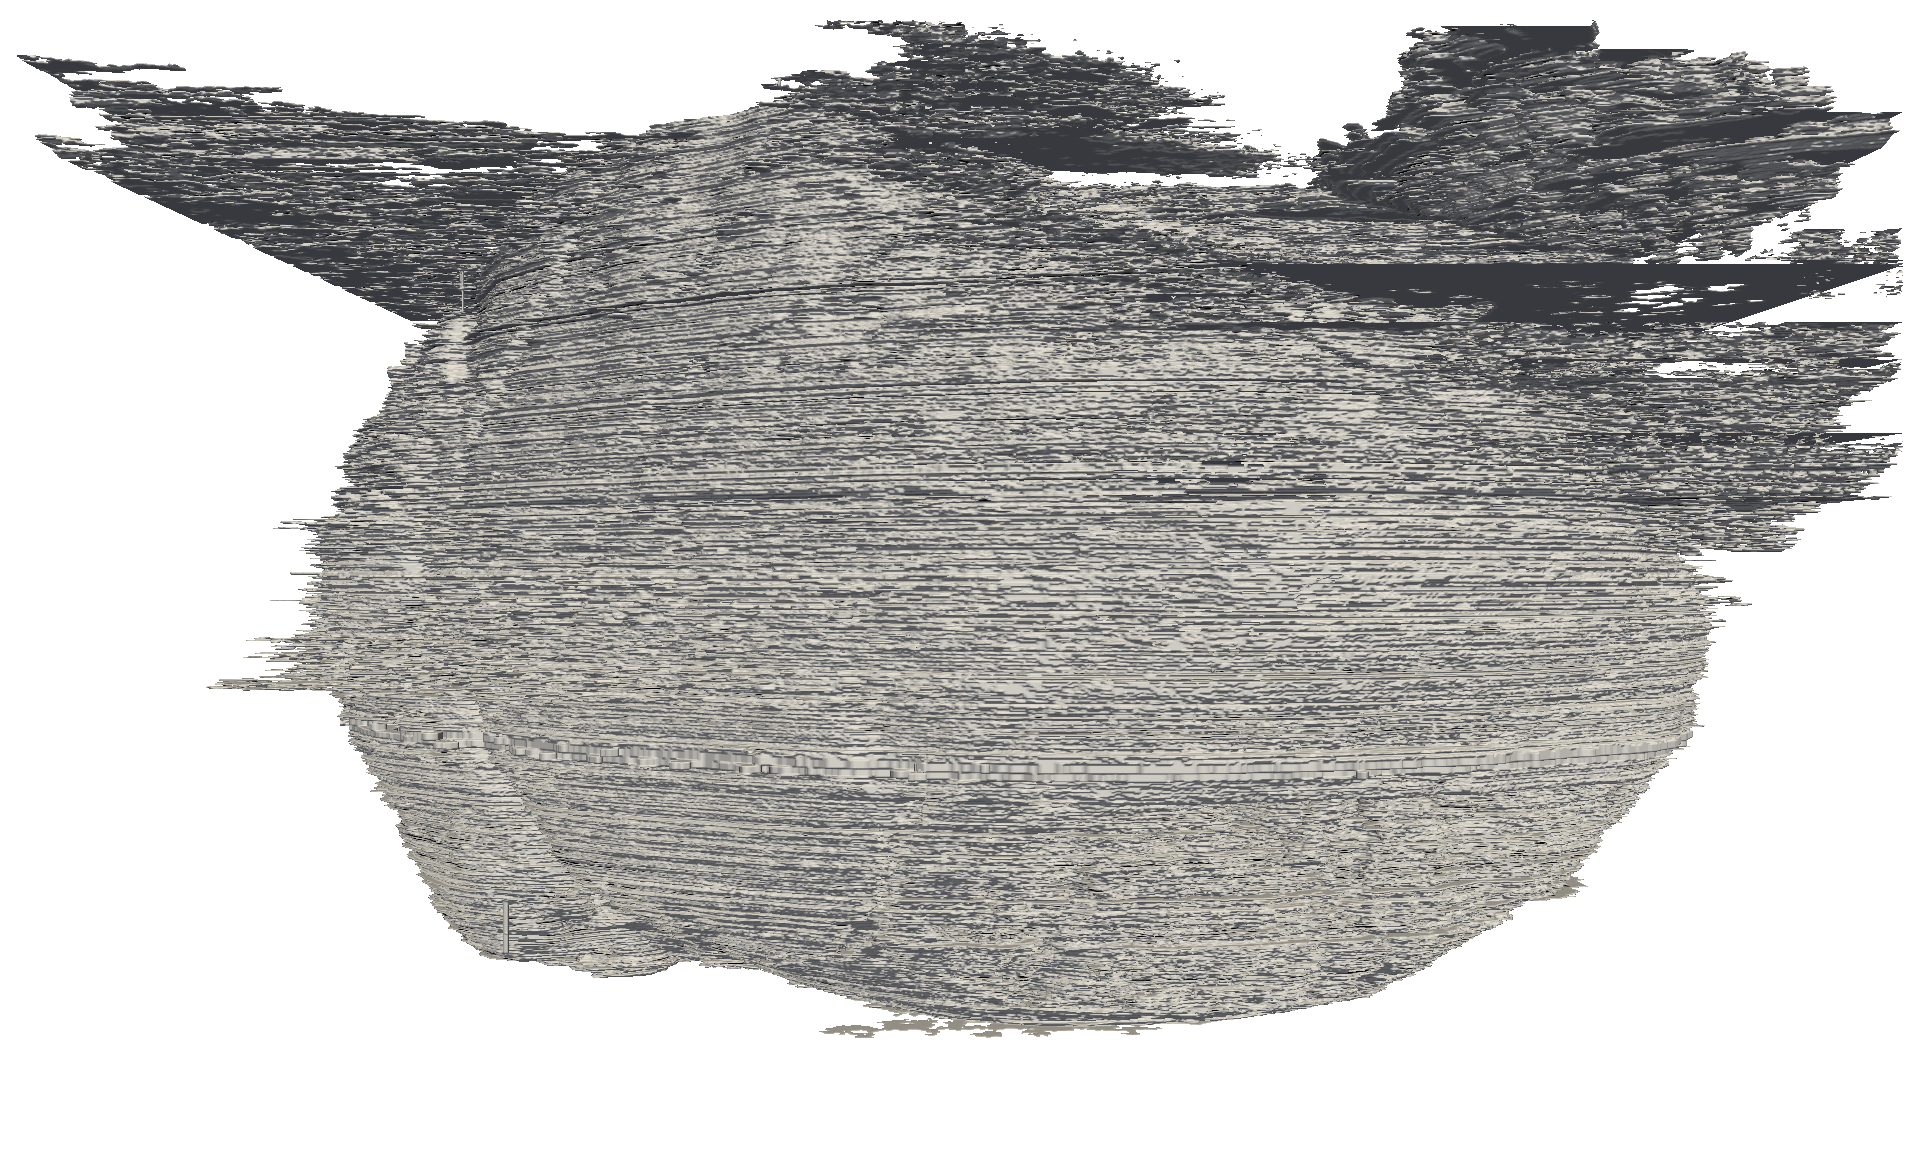
\includegraphics[width=\textheight]{Ch5/Figs/Rat28/contours/LoRes_positive_x}
      \caption{A contour of the adjusted block face volume, viewed along the positive x direction. The round surface of the heart apex is clearly visible to the right. Oddly shaped protrusions in the top third of slices are due to gradually brightening reflection from the suface of the wax.}
      \label{fig:LoRes_positive_x}
    \end{sidewaysfigure}
    
    \begin{sidewaysfigure}[htbp]
      \centering
      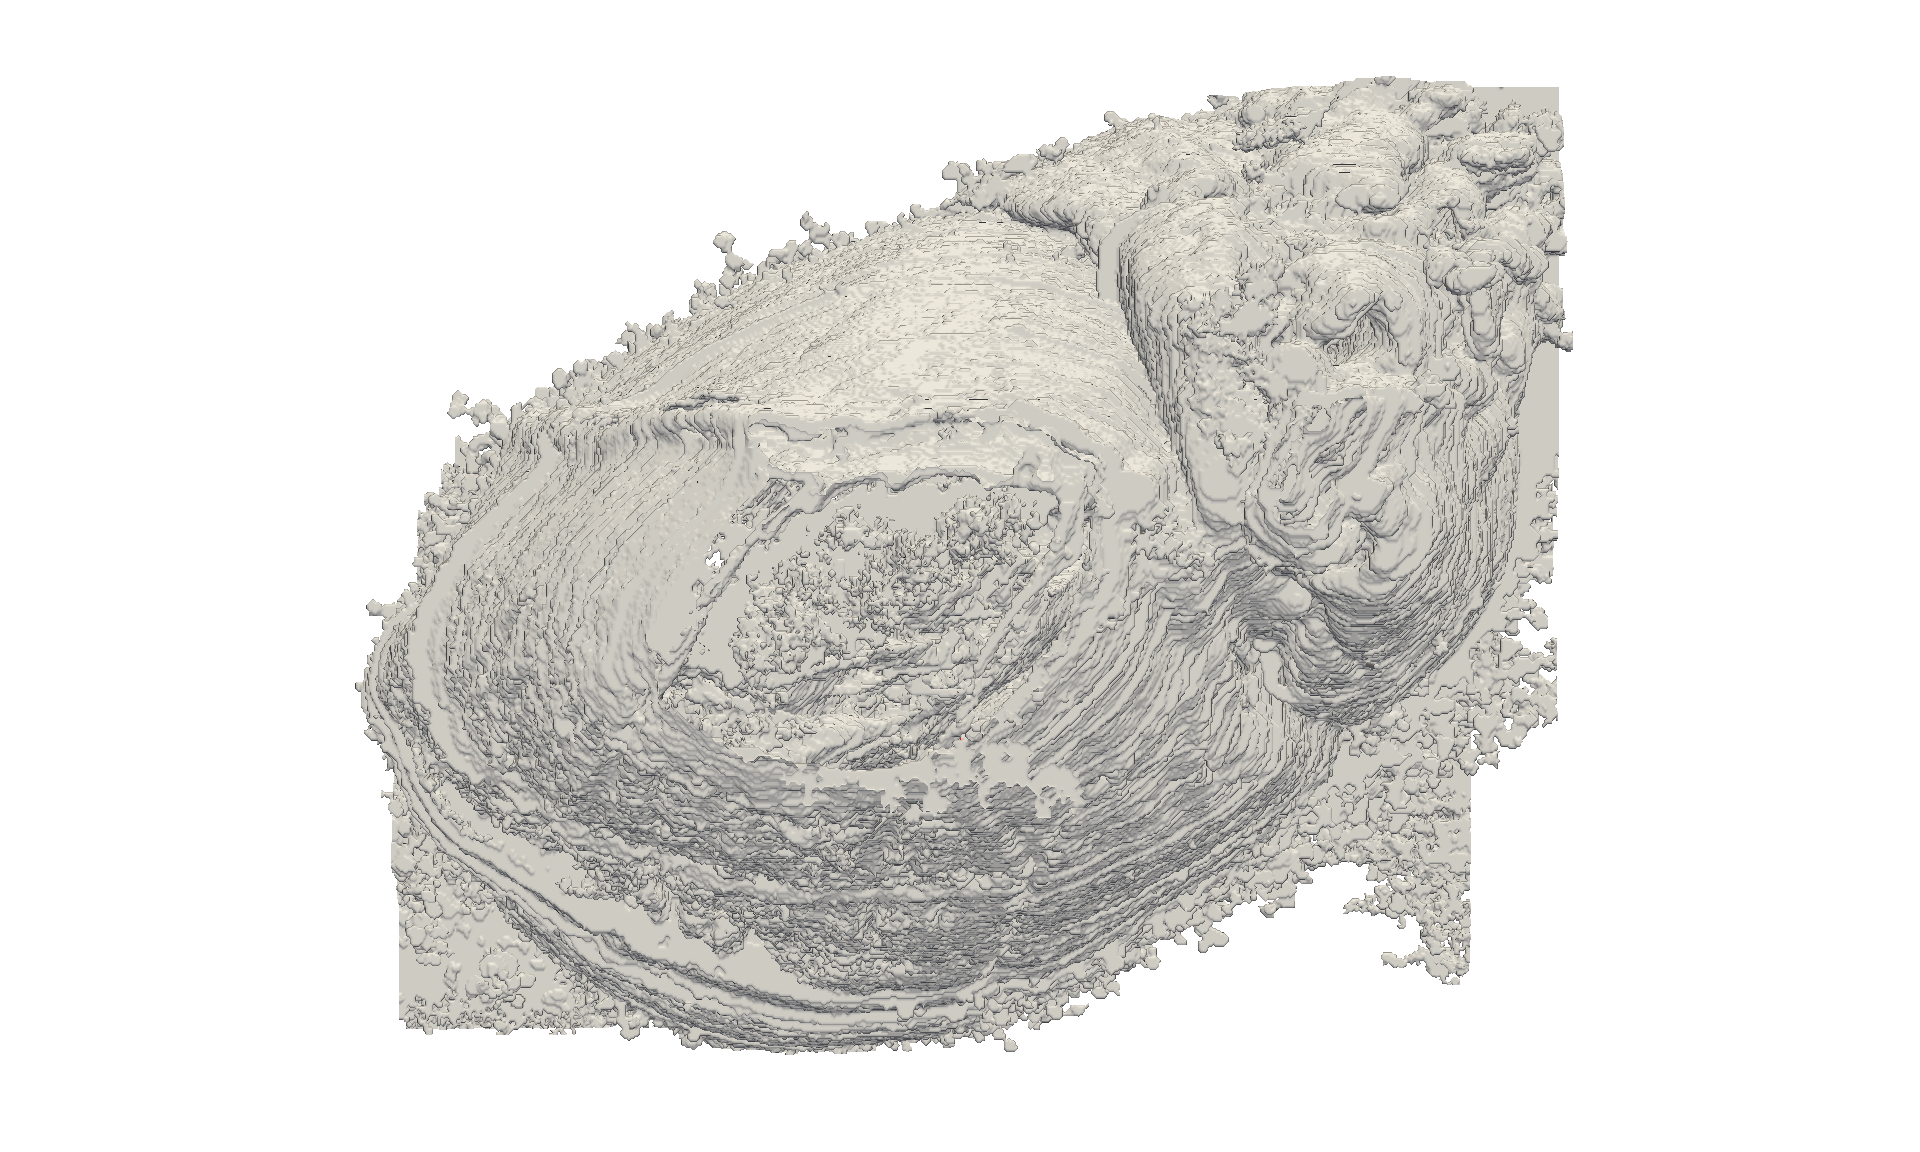
\includegraphics[width=\textheight]{Ch5/Figs/Rat28/contours/LoRes_positive_z}
      \caption{The block face contour viewed along the positive z direction. The detail and composition of the images is clearly visible from this angle. Note the protruding epicardial vessel in the top left. The surface of the first third of slices near the bottom left looks eroded, in a region where the threshold intensity values have failed to pick up the tissue boundary faithfully.}
      \label{fig:LoRes_positive_z}
    \end{sidewaysfigure}
    
	As is evident from Figures~\labelcref{fig:original_lores_images,fig:original_hires_images} for one slice, the vast majority of slices had been flipped over between sectioning from the block surface and being photographed. Slice images were therefore reflected across one axis in order to restore geometric parity with the associated block face image.
	
	 Several sets of downsamples of varying factors were generated, the lowest of which were used for debugging and testing, working up in detail, size and computational expense as the techniques were perfected. Before downsampling, a Gaussian smoothing was applied in each case, with sigma equal to the new larger pixel spacing. In this way, all original pixels in the region of a large downsampled pixel contribute to its final value, and aliasing noise problems associated with frequencies higher than half the downsampled pixel spacing are avoided. This results in a smoother and more accurate cost function. Figures~\labelcref{fig:original_lores_images,fig:original_hires_images} juxtapose the full images with various levels of downsampling.
	 
	 When registering two images, it is important that they are of comparable resolution, in order to minimise processing time and to ensure the smoothest possible cost function. In Figure~\ref{fig:downsample_zooms}, the effects of the downsampling can be seen more clearly. Individual cell nuclei are resolved at the highest resolution of slice image, but the maximum resolution block face images are of much lower detail. Clearly, the original slice images, with 1.1$\mu$m pixel spacings, are needlessly detailed compared to their block face counterparts, with a mere 26.6$\mu$m. As is discussed in Section~\ref{ssub:multiresolution_registration}, it is therefore appropriate to register slice images at a factor of 8 times more downsampled than the block face images.
    
	%  Lo/HiRes zooms
    \begin{sidewaysfigure}[htbp]
      \centering
      \subfigure[][]{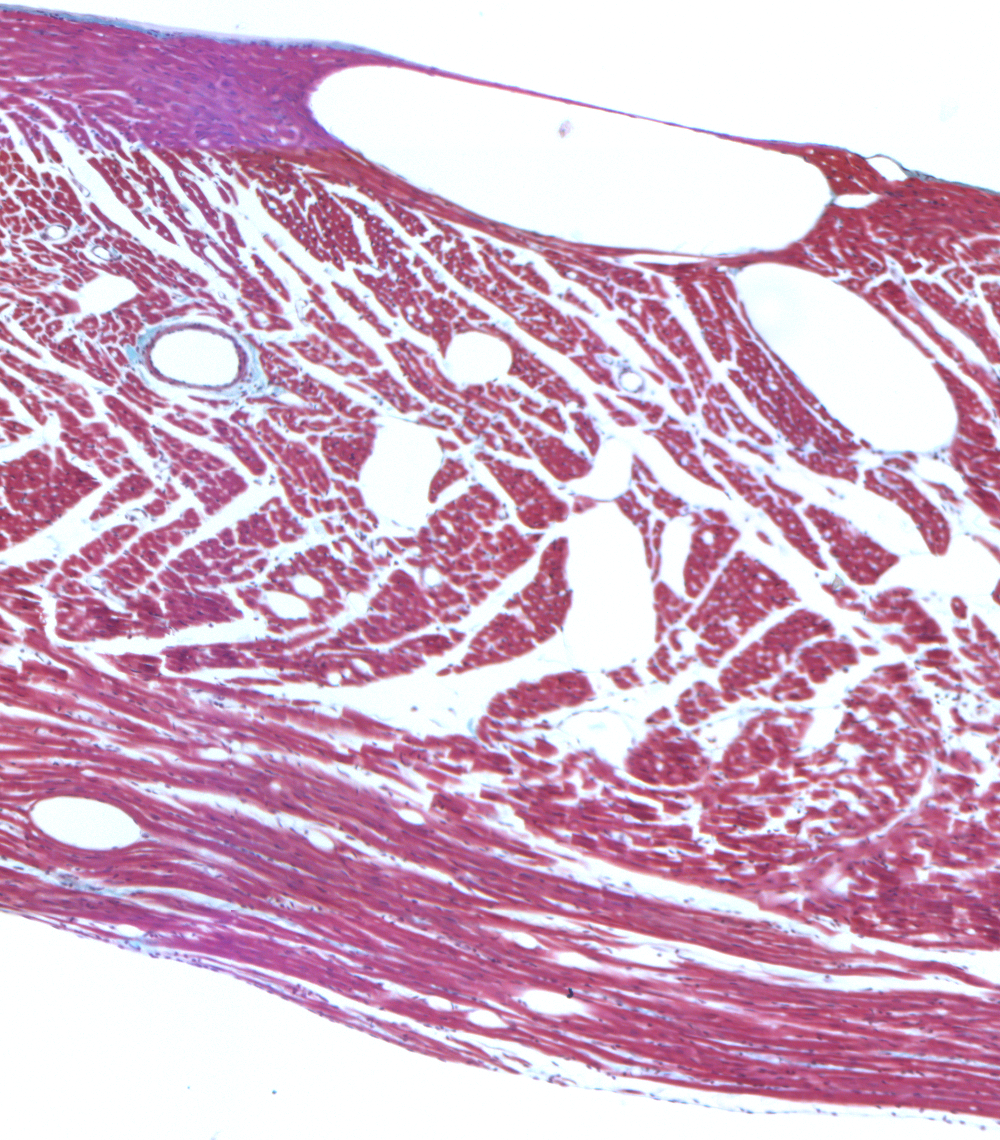
\includegraphics[width=0.39\pagewidth]{Ch5/Figs/HiRes_downsamples_1_0582_zoom}}
      \subfigure[][]{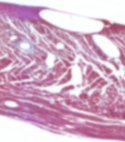
\includegraphics[width=0.39\pagewidth]{Ch5/Figs/HiRes_downsamples_8_0582_zoom}}
      \subfigure[][]{
\includegraphics[width=0.39\pagewidth]{Ch5/Figs/HiRes_downsamples_64_0582_zoom}}
      \subfigure[][]{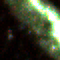
\includegraphics[width=0.39\pagewidth]{Ch5/Figs/LoRes_rgb_downsamples_1_0582_zoom}}
      \subfigure[][]{
\includegraphics[width=0.39\pagewidth]{Ch5/Figs/LoRes_rgb_downsamples_8_0582_zoom}}
      \caption{An epicardial vessel in slice 582 of Rat 28, in both the slice and the block face images. \textbf{(a)}, \textbf{(b)} and \textbf{(c)} show the slice original, 8x and 64x downsampled, while \textbf{(d)} and \textbf{(e)} show the block face original and 8x downsampled. The fibres parallel to the internal wall at the bottom of \textbf{(a)} are angled such that they reflect the illumination strongly at the top right of \textbf{(d)}, and are in much sharper contrast to the black wax than the rest of the tissue. Indeed, they are in much sharper contrast to the other tissue than the other tissue is to the non-tissue.}
      \label{fig:downsample_zooms}
    \end{sidewaysfigure}
  % subsection image_preparation_and_curation (end)
  
  \subsection{Initialisation} % (fold)
  \label{sub:initialisation}
    The optimisation algorithms used in registration do not assure convergence to the global minimum and are thus sensitive to initialisation and to the presence of local minima in the cost function. A reasonable initialisation is necessary for robust and accurate registration.
	
		\subsubsection{Geometric Initialisation} % (fold)
		\label{ssub:geometric_initialisation}
			The block face images are already coherent from their acquisition. White space under the microscope surrounding the slices had already been cropped, such that each slice sat approximately centrally within the bounds of its image. Having been reflected across the x-axis, an anticlockwise rotation of $90\,^{\circ}$ oriented most slices approximately with the block face, as is seen from Figures~\labelcref{fig:original_lores_images,fig:original_hires_images}. A small set of slices required $180\,^{\circ}$ rotations. Slice images were then initialised to their common centre to form a volume. The initial translation and pixel spacing of the block face volume was then manually tuned to overlap maximally with the slice volume. As is exhibited in Section~\ref{sec:results}, this na\"ive geometric initialisation provides an adequate starting point.
		% subsubsection geometric_initialisation (end)
	
		\subsubsection{PCA Initialisation} % (fold)
		\label{ssub:pca_initialisation}
			Although geometric initialisation provided a reasonable starting point for most slices, this was purely a consequence of how the experimentalist had manually obtained and cropped the original images. A more sophisticated method might make use of the information in the image. If the pixels containing tissue could be identified, the centres of mass and principal components of each pair of images can be aligned to provide a close initial matching.
		
		  Various segmentation methods were tested in an effort to identify tissue reliably in both sets of images. Because the block face volume was already coherent, volume-wise refinements and filters could be applied, whilst only 2D segementation techniques could be considered for the slice images.
			
			After applying any image preprocessing, such as a gradient magnitude or Hessian filter, many segmentation methods, such as opening and closing or level sets, are designed to refine the edges or surfaces of an approximate segmentation. Yet here it is to be noted that only the segmentation's moments are of consequence, in particular the centre of mass and the variance matrix. It is therefore unnecessary for the segmentation to overlap closely with the tissue at a small scale, only that the global distribution of tissue be represented precisely. That being said, methods to remove macroscopic artefacts, such as connected component filtering and selection proved beneficial in most contexts.
			
		  There is no facility to align the principal components of two images in ITK, only to align their centres of mass. The class itk::CenteredTransformPCAInitializer was implemented to encapsulate the details of this process. The results of applying this class compared to the simple geometric initialisation are shown in Figure~\ref{fig:582_pca}, and the segmentations upon which they are based are shown in Figure~\ref{fig:582_segmentation}.
		
	    It is somewhat clear from Figure~\ref{fig:LoRes_cross_sections} that the broad range of tissue colours and intensities in the block face volume overlap significantly with the colours and intensities of non-tissue. In Figures~\labelcref{fig:582_segmentation,fig:582_pca}, the threshold segmentation values were optimised for these particular slices as a proof of concept, but this slice was chosen as one of the best examples of the technique. Issues such as wax bubbles, the bright blob at the top of the block face volume, optical transmission from layers below, and differential brightness from differing fibre directions or anatomical features plagued efforts to segment the images, and in fact went on to plague registration. Even if a segmentation method could yield reasonable results for every slice in the dataset, it is impractical to tune parameters manually for each slice, and there would certainly not be a single parameter set suitable for every slice in the volume. For these reasons, the PCA method could not be used to improve robustly upon a simple geometric initialisation of the high-resolution slices seen in Figure~\ref{fig:geometric_initialisation}.
    
	  \begin{figure}[htbp]
	    \centering
      \subfigure[][]{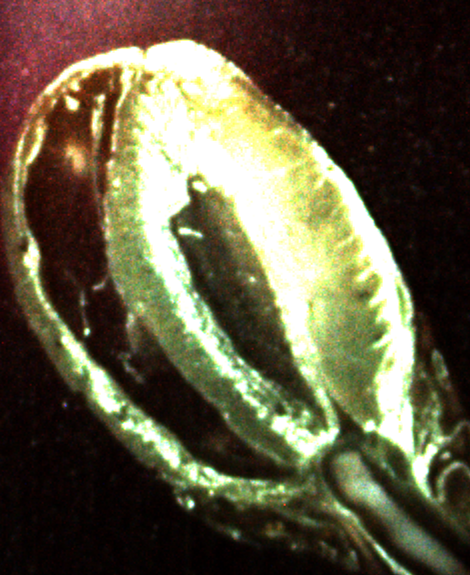
\includegraphics[width=0.4\pagewidth]{Ch5/Figs/pca/LoRes_562}}
      \subfigure[][]{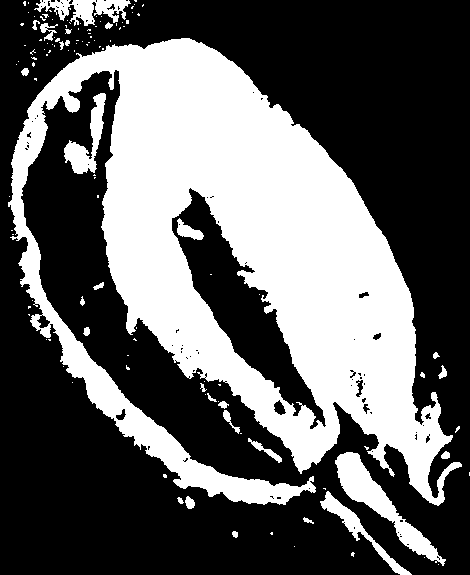
\includegraphics[width=0.4\pagewidth]{Ch5/Figs/pca/LoRes_segmentation_562}}
      \subfigure[][]{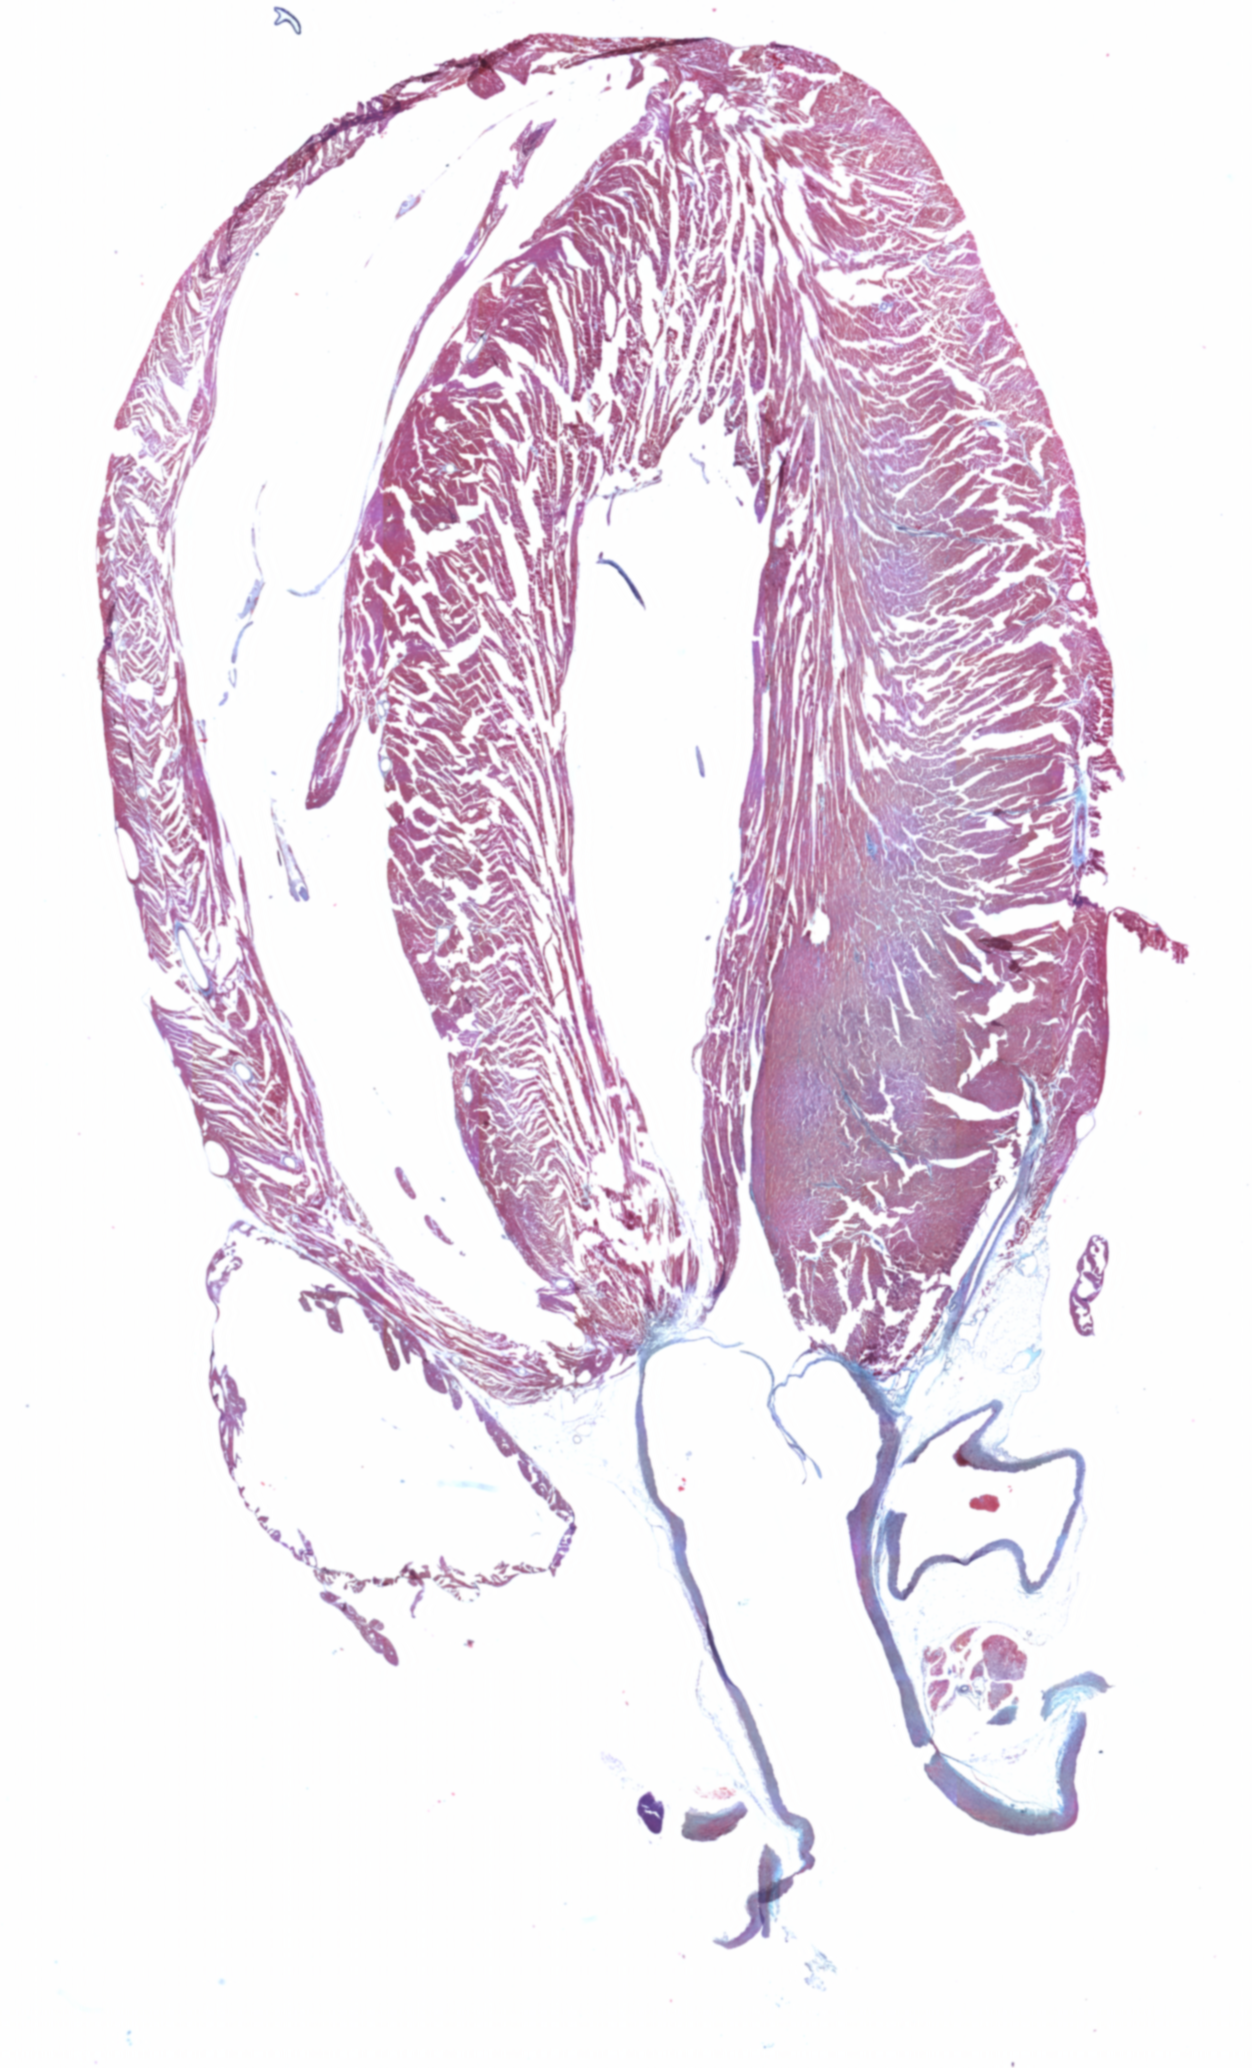
\includegraphics[width=0.4\pagewidth]{Ch5/Figs/pca/HiRes_562}}
      \subfigure[][]{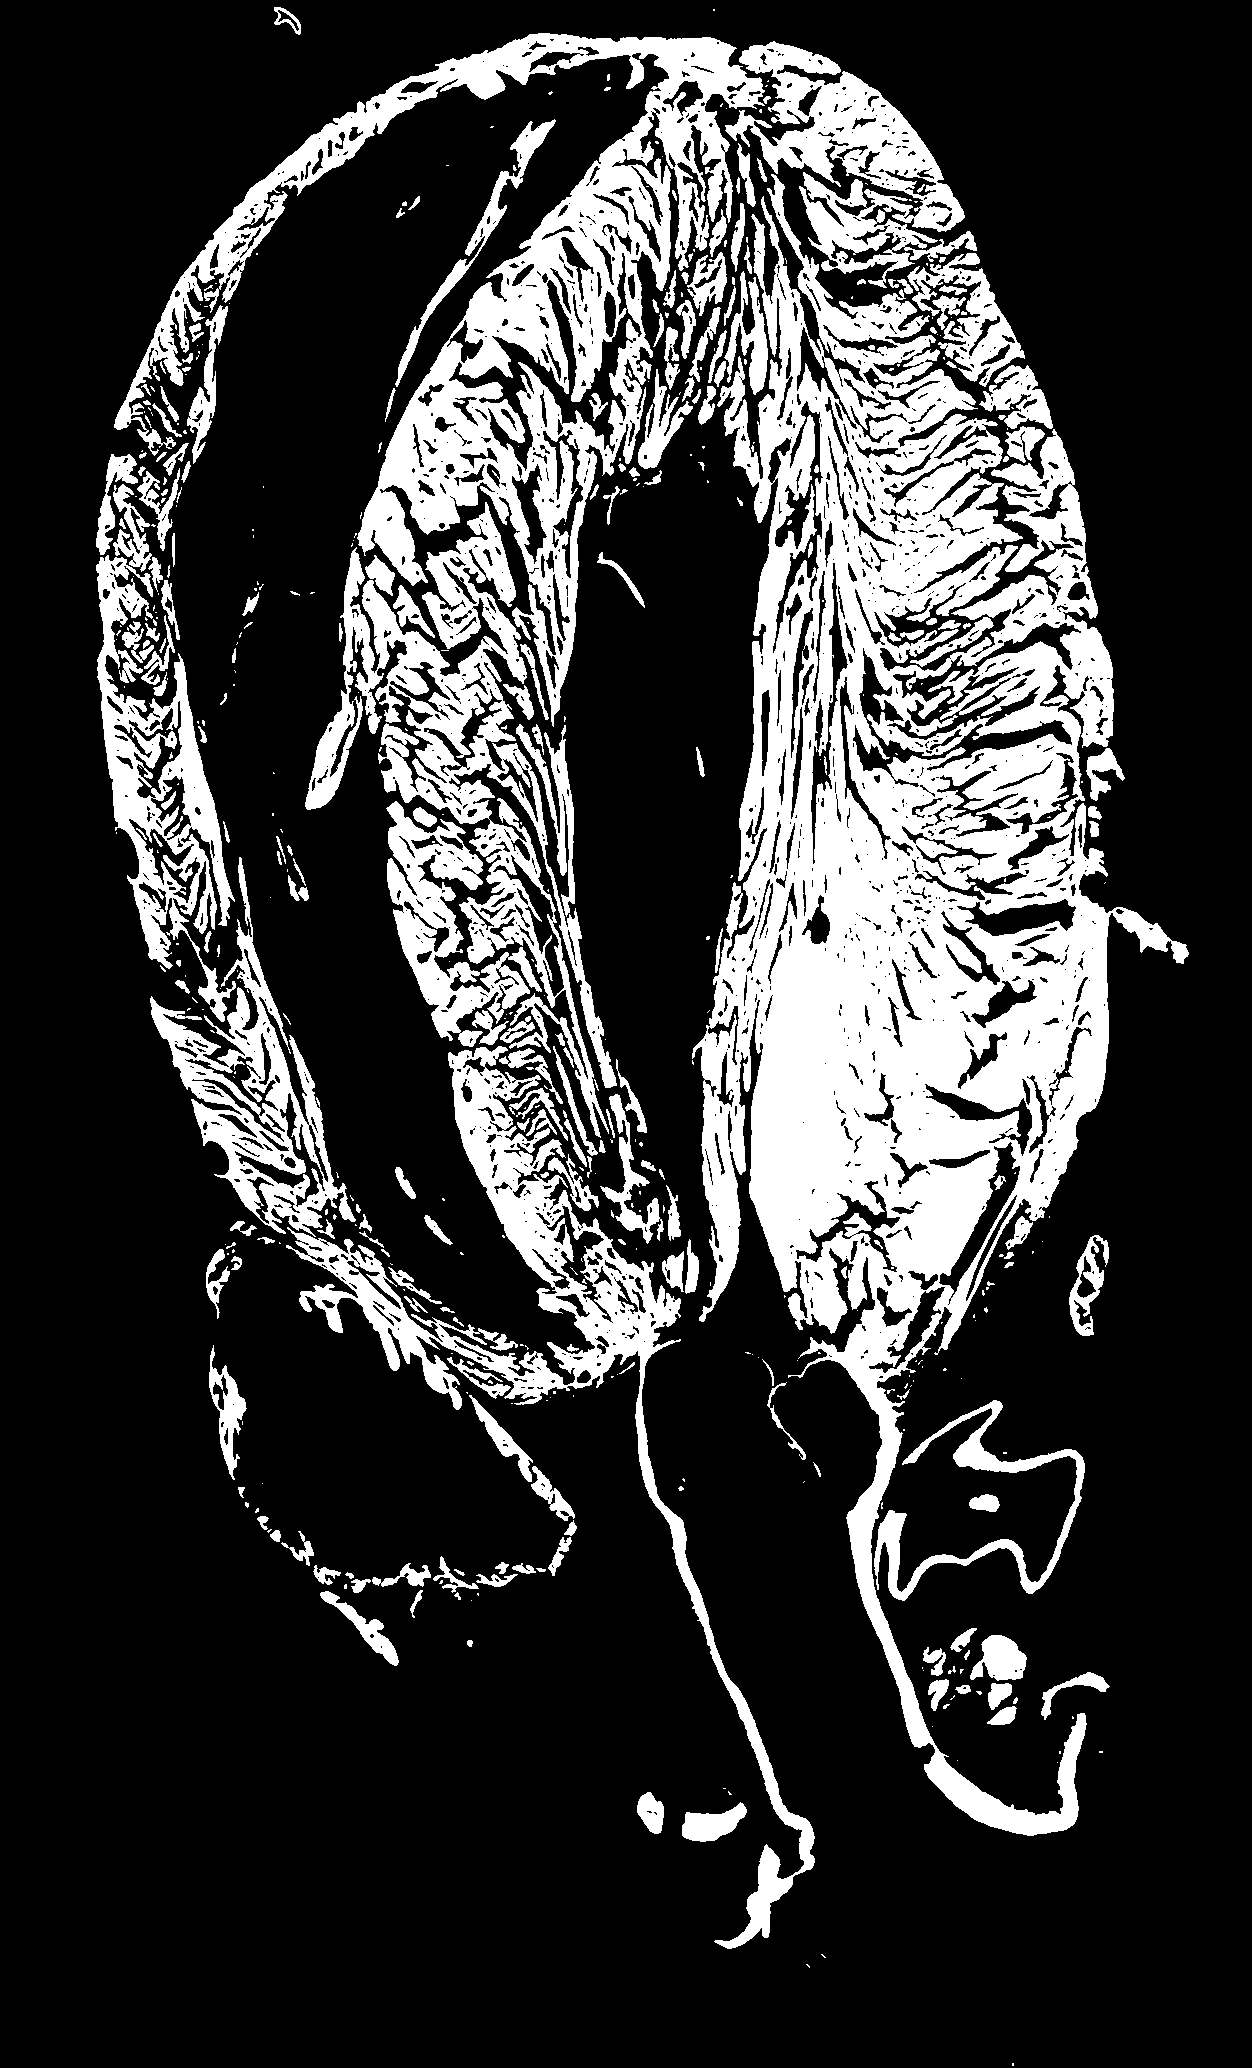
\includegraphics[width=0.4\pagewidth]{Ch5/Figs/pca/HiRes_segmentation_562}}
      \caption{Originals and threshold segmentations of the block face and slice images of slice 582.}
	    \label{fig:582_segmentation}
	  \end{figure}
    
	  \begin{figure}[htbp]
	    \centering
      \subfigure[][]{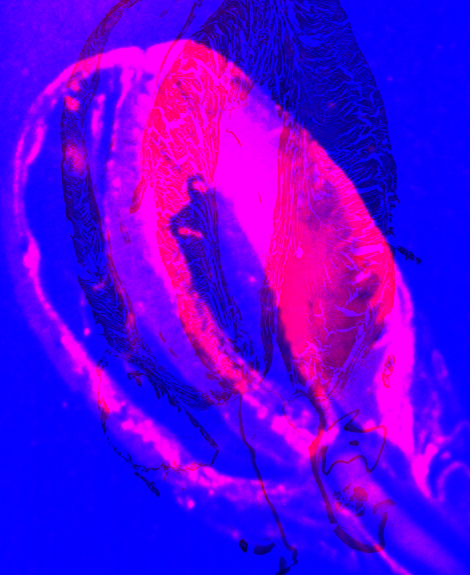
\includegraphics[width=0.4\pagewidth]{Ch5/Figs/pca/geometric_redblue}}
      \subfigure[][]{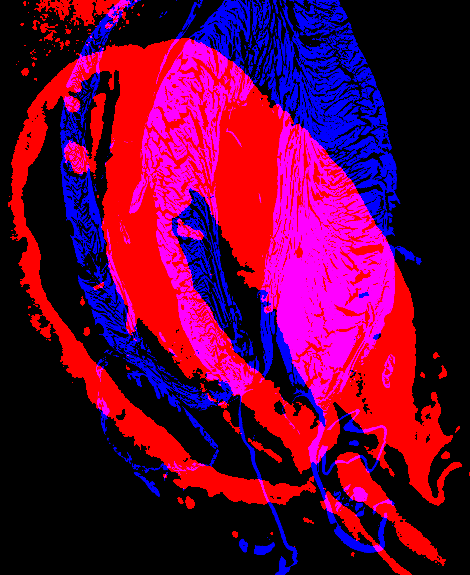
\includegraphics[width=0.4\pagewidth]{Ch5/Figs/pca/geometric_segmentation_redblue}}
      \subfigure[][]{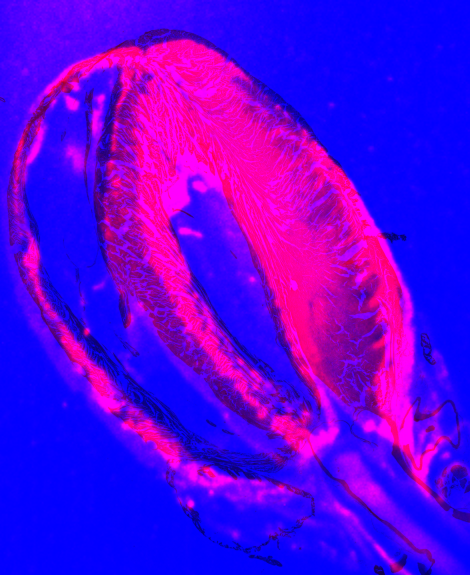
\includegraphics[width=0.4\pagewidth]{Ch5/Figs/pca/pca_redblue}}
      \subfigure[][]{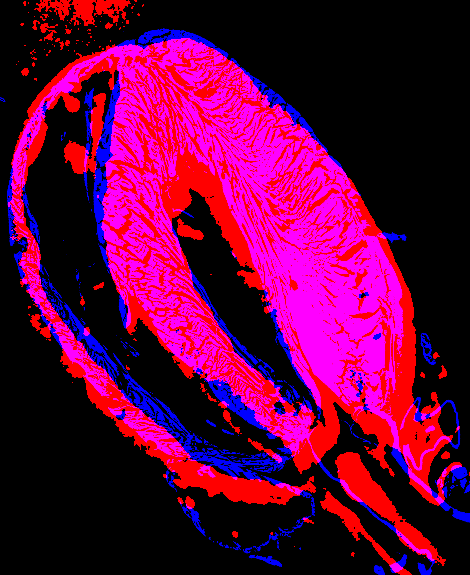
\includegraphics[width=0.4\pagewidth]{Ch5/Figs/pca/pca_segmentation_redblue}}
      \caption{Intensity superpositions of block face (red channel) and slice (blue channel). The original images are used \textbf{(a)} and \textbf{(c)}, while the segmentations are shown in \textbf{(b)} and \textbf{(d)}. \textbf{(a)} and \textbf{(b)} show geometric initialisation, and \textbf{(c)} and \textbf{(d)} PCA initialisation. It is clear that PCA provides a much closer match from which the registration algorithm can begin.}
      \label{fig:582_pca}
    \end{figure}
    
		% subsubsection pca_initialisation (end)
  % subsection initialisation (end)
  
	\subsection{Registration Algorithm} % (fold)
  \label{sub:registration_algorithm}
    Each main aspect of the registration method is outlined in this section. A well-founded registration algorithm must embody three traits: numerically, it must converge reliably to the global minimum; computationally, it must be efficient so as to be tractable; and physically, it must correspond to the process that it was designed to correct for. It is through the lens of these three benchmarks that we examine the following components.
    
    \subsubsection{Transforms} % (fold)
    \label{ssub:transforms}
			The sectioning of the slices introduces 2D, slice-specific deformation and in some cases damage. The subsequent relaxing and rehydration of each slice causes further deformation. A large proportion of this deformation will be of similarity or affine form. By first registering the simplest of transforms with the lowest dimensional parameter space, and then incrementally relaxing transformational constraint by increasing the number of parameters, we can provide the best possible starting point in each higher dimensional parameter space.
			
      Transforms were optimised in the following order, the final result of each initialising its successor: a centered rigid 2D transform - a rotation about an arbitrary centre followed by a translation; a centred similarity transform - as before but with a scaling factor; and a centred affine transform - an affine transformation around an arbitrary centre followed by a translation. For all transforms, the centre of rotation was exposed for optimisation as metric parameters. Finally, a coarse grid and subsequent fine grid bspline deformable transform was tested, but found to be unstable.
    % subsubsection transforms (end)
    
    \subsubsection{Metrics} % (fold)
    \label{ssub:metrics}
      Mutual Information (MI) is usually considered to be most effective when registering images from different modalities. However, after a plethora of parameterisations and configurations was explored based on this metric with little success, incrementally simpler and simpler metrics were tested. Each demanded more image preconditioning and tuning, but yielded monotonically closer and more consistent registrations, with a larger capture range, and required fewer iterations to converge. First, a normalised correlation was employed, with the simplest mean squares difference algorithm proving most suitable. It would appear that the simpler the intensity relationship, the smoother the cost landscape, with fewer local minima.
    % subsubsection metrics (end)
  
    \subsubsection{Optimisation} % (fold)
    \label{ssub:optimisation}
      Gradient Descent (GD) and Regular Step Gradient Descent (RSGD) optimisers have been applied. RSGD terminates before the maximum number of iterations has passed, and so in simple cases it is computationally more efficient. In most scenarios, however, the GD optimiser often proves more robust. In both cases, a choice to maximise or minimise the cost function must be chosen, the latter being dependent on both the choice of metric and the preconditioning of the image intensity ranges.

      The optimisation space, as dictated by the transform, must be scaled along each dimension to correct for discrepant effects per unit change of each parameter. For example, a translation of one micron at the epicardium might result from a rotation of just $10^{-5}$ radians about the centre of the slice. This makes the metric space more isotropic and reduces the eccentricity of cost function basins, allowing the optimisation algorithm to fall more directly toward minima.
    % subsubsection optimisation (end)
	% subsection registration_algorithm (end)
    
  \subsection{Software Architecture} % (fold)
  \label{sub:software_architecture}
		From early on, the requirements of the problem diversified, and a range of related tools were built. Common patterns and functionality needed to be extracted and isolated. This prevented duplication and the potential for bugs and inconsistencies, and lead to more readable and manageable code. Because the final result was unknown, it was often extremely difficult to know whether the code was operating correctly. Bugs or errors in calculation were not usually apparent, and proved very difficult to find. We outline the main problems encountered during the development process, along with the solutions crafted to isolate and overcome them.
		
		\subsubsection{Languages and Frameworks} % (fold)
		\label{ssub:languages_and_frameworks}
      All file handling and networking algorithms were written in Ruby. Imaging algorithms were written in C++ or, in some simple cases, Python, using the venerable ITK library. C++ executables were compiled using the cross-platform build system CMake. YAML was used as a declarative language for configuration files, providing a syntax that is easily human readable and curatable, yet machine parsable. Source code management and code deployment was implemented in Git, and the project is freely available at \url{http://github.com/mattgibb/registration} under an MIT license.
		% subsubsection languages_and_frameworks (end)
		
    \subsubsection{Stacks} % (fold)
    \label{ssub:stacks}
      Each block image must be paired with its equivalent slice image, and blank images must be interpolated where images are missing. Slices must be transformed independently and by a range of transform types. Resampler spacings must be set according to the original image spacings and the downsample ratios. Binary masks must be generated for each image, so that metrics will only take pixel intensities into account from inside the boundaries of the original untransformed images. A stack volume must be reconstructed from the transformed, resampled slices. A minimum percentage overlap is required for many metrics to function, and for small slice images close to the apex of the heart, block mask areas must be cropped until this constraint is satisfied.
	  	
      A hierarchy of Stack classes has been developed - along with associated builder classes, IO helpers and transform converters - to encapsulate the solutions to all of these problems. A Stack represents the 3D composition of a set of 2D slices. It handles ROI selection, generic transform storage, image and mask resampling and generation (both for 2D slices and for the 3D volume) and various error handling strategies. An MRI class is also available to solve the complementary problem of extracting arbitrarily oriented slices from a 3D image. However, for these specific datasets the block face images are intrinsically registered to the histological samples.
    % subsubsection stacks (end)
    
    \subsubsection{Multiresolution Registration} % (fold)
    \label{ssub:multiresolution_registration}
			The total size of the block face and slice images approaches two terabytes \cite{Gibb2012} and pose significant challenges for computational processing and visualisation \cite{Goodyer2009}. Even with an 8x downsampled slice dataset, one full rigid registration to test one parameter set would take nearly 100 hours on a modern quad core processor. An affine registration performed with a regular step gradient descent optimizer is parameterised in 10 dimensions. Rapid feedback is required if the right parameters are to be found in any reasonable time, and so a multiresolution approach must be taken. There are 2 ways to reduce the resolution of the dataset: in-plane downsampling and out-of-plane slice selection.
			
      In-plane downsampling and Gaussian smoothing not only reduces time, but smooths the cost function and can lead to more robust registration results. In multiresolution registration, the resulting transforms can then be used to initialise a more accurate but more fragile registration at a higher resolution.
			
      To start with, a quick order-of-magnitude overview of the global performance of a particular parameter set was required. In this case, regularly spaced subsets of the full curated list were created, such as every thirtieth slice or every fifth slice. Alternatively, every slice within a region might be selected, for example, the band of slices spanning an epicardial vessel. Of course, these two reductions can be applied together for very rapid feedback. As will be made clearer in Chapter~\ref{cha:diffusion_smoothing_registration_of_high_resolution_rat_histology}, full out-of-plane resolution is required to parameterise effectively the coregistration of adjacent slices. However, the fruitful region of parameters near the apex of the heart for elliptical discs of tissue is different (yet not disjunct) from that in more complex, central slices. In this case, a group of representative slice sublists at full resolution, e.g. 100-110, 200-210, 300-310 etc., provide the best compromise between speed and accuracy.
			
			The slice list is loaded dynamically by all tools from a central config file, and so switching between lists when prototyping is as simple as redirecting a symlink.
    % subsubsection multiresolution_registration (end)
    
    \subsubsection{Builders} % (fold)
    \label{ssub:builders}
      A minimal registration pipeline is composed of several generic actors, including a metric, an optimiser, a transform, and an interpolator. The details of which types of actors are optimal and how they should interact are peculiar to the registration problem at hand. Furthermore, the specific type of each component often requires unique configuration beyond the generic interface of its family, and the choice of image preprocessing is dependent on the choice of metric. Once several types must be chosen from and configured, even for just one component, an ad hoc procedural approach quickly became unwieldy. These two requirements colluded combinatorially to demand a great deal of testing, tailoring and configuration in order to achieve registrations of high quality. More often than not, modifications would degrade the registration.
			
      The `Gang of Four' proposed the first categorised set of recurring solutions to common problems in object-oriented software design \cite{Gamma1995}. Three patterns they introduce are the Builder Pattern, the Abstract Factory Pattern and the Strategy Pattern. The Builder Pattern and the Abstract Factory Pattern are closely linked, both in their purpose and in their implementation; the Builder Pattern focusses on the construction of a single, complex object, whilst the Abstract Factory Pattern constructs a family of related or dependent objects. The Strategy Pattern encapsulates a group of concrete algorithms behind a generic interface, and makes them interchangeable with respect to any application code that employs them.
      
      At the pipeline level, we developed a hierarchy of frameworks employing the Builder pattern (\cite{Gamma1995}), whose purpose is to abstract away the heavy lifting of wiring up the various components together. At the component level, a conflation of the Abstract Factory and the Strategy patterns (\cite{Gamma1995}), together with a configuration system using the human-friendly YAML markup language, serves not only to decouple the actors' representations from the minutiae of their construction, but to move these volatile decisions from compile-time to runtime. These tools vastly reduce the cost of experimentation and testing. With all the variables clearly grouped together, with no need to recompile the toolchain or pore through source code to find if and where one can make a change, the feedback from results is faster and less error prone.
      
			The StackAligner class encapsulates the registration process, for tools employing affine or b-spline deformable transforms, across the whole heart or in a region of interest. At least two sets of stack configurations were required, for the block face and slice stacks, across a great many registration and reconstruction tools. This logic was pulled into a StackBuilder class tree, rooted from an untemplated StackBuilderBase class to prevent template infection across the codebase.
    % subsubsection builders (end)
		
		\subsubsection{Events, Checkpointing and IO} % (fold)
		\label{ssub:events_checkpointing_and_io}
			It is necessary to save intermediate information about the progress of the registration, for parameter tuning and analysis. ITK exposes this functionality through the Command Observer pattern (see \cite{Gamma1995})). Any ITK object can publish events, and other objects may subscribe to those events. An object whose purpose is to subscribe to an event and perform an action when that event is triggered is called a Command Observer. Figure~\ref{fig:command_hierarchy} shows the class tree developed to display and record the required information.
			
    \begin{figure}[htbp]
      \centering
      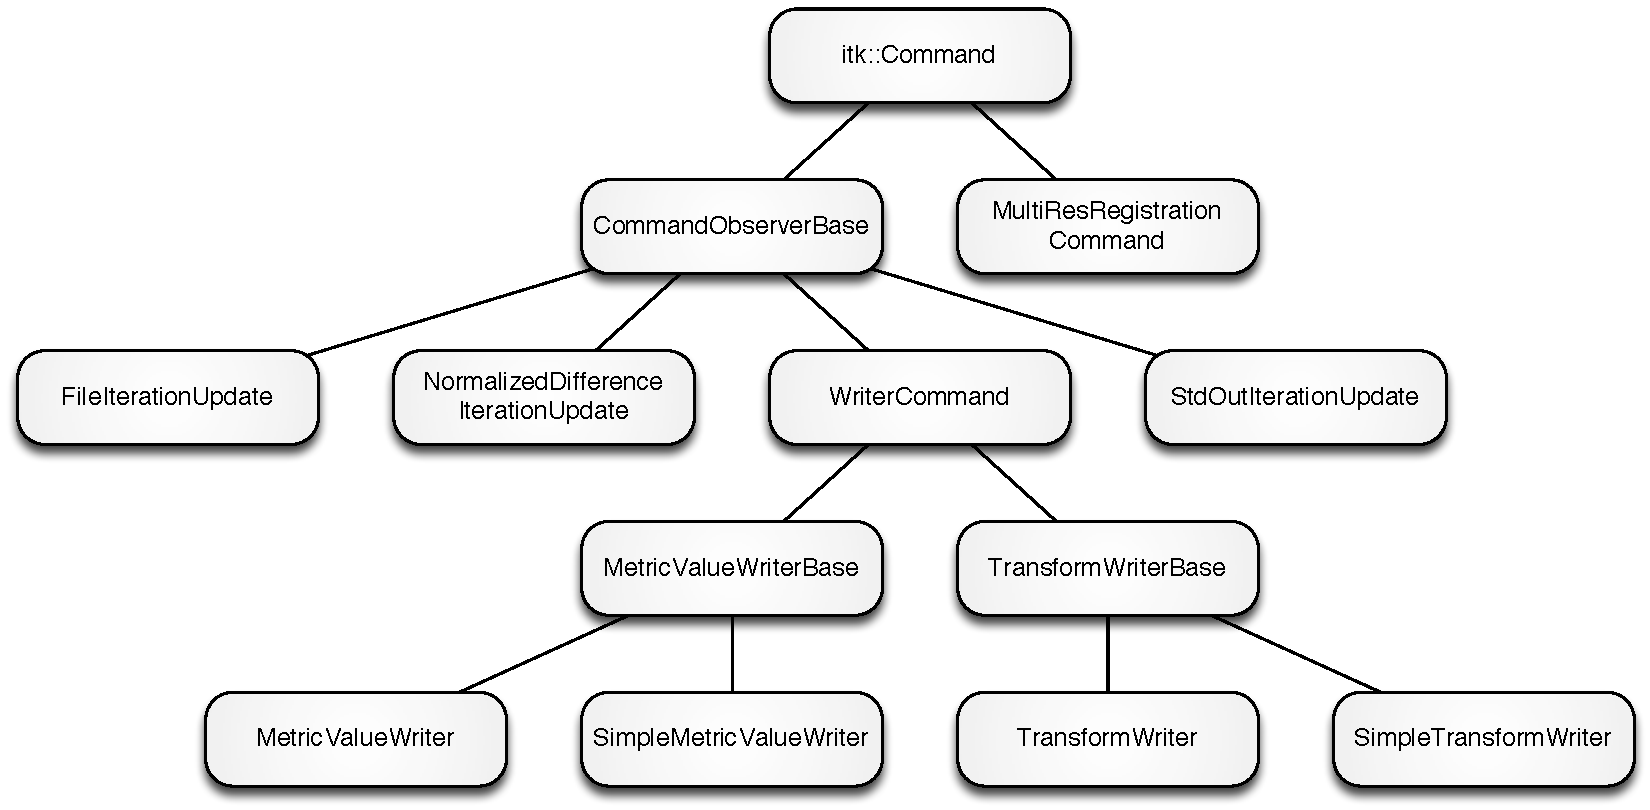
\includegraphics[width=\pagewidth]{Ch5/Figs/command_hierarchy}
      \caption{Command Observer hierarchy to output various types of information when specific events are triggered.}
      \label{fig:command_hierarchy}
    \end{figure}
		
      At any stage during the registration process, the vector of transforms held by a given Stack can be persisted to a series of files with a single function call. Just as easily, a new Stack can be initialised with a set of transforms on storage. This machinery facilitates greater process granularity in three dimensions: in the sequence of transforms to be optimised, in the increasing image resolutions to be registered, and spatially in the pairs of slices within the Stack. In the first case, a user can tune one registration stage until they are happy that it is optimal, and then use the results as a starting point for all subsequent runs of the next stage. In the second case, approximate registrations can be performed with images at lower resolutions, which can then initialise registrations at higher resolutions with different images. In the third case, the result from separate jobs for each slice pair using images of a scalar floating point pixel type or a segmentation image type can be aggregated and used to reconstruct a colour volume, perhaps at a different resolution. This division of workload and memory is of particular importance when organising jobs on clusters and shared memory machines.
			
			Even aside from process granularity, working with transforms is vastly superior to working directly with the images. Composing transforms rather than repeatedly resampling prevents a loss of image quality due to rasterisation in differing coordinate systems. Advanced composition of transforms makes possible registration refinement, either in regions of interest, or with the diffusion smoothing techniques discussed in Chapter~\ref{cha:diffusion_smoothing_registration_of_high_resolution_rat_histology}.
          
          Several other aspects of the architecture are not discussed here, including configuration, file management, testing, as well as the opportunities and challenges posed by high performance computing.
		% subsubsection events_checkpointing_and_io (end)
		
  % subsection software_architecture (end)
  
  \subsection{Diagnostics and Parameter Tuning} % (fold)
    \label{sub:diagnostics}
      For almost a year and a half, it was very difficult to see why registration was failing to yield robustly accurate results. The output of raw parameters was somewhat elucidating, but only for obvious issues such as parameter scaling and step length, where almost zero change in some or all parameters signalled what to adjust. The space of possible parameters was enormous, and the computing time before feedback significant. With visual representation of nothing but the final result, determining which parameters to change and how was perhaps analogous to deciding how each player in a sports team could improve given only the final scores.
      
      Armed with the intermediate transforms and metric values discussed in Section~\ref{ssub:events_checkpointing_and_io}, the causes of the suboptimal registration results were immediately apparent. The progression of metric values for all slices could be plotted in graphs like those in Figures~\labelcref{fig:rigid_metric_values,fig:similarity_metric_values,fig:affine_metric_values,fig:affine_metric_value_differences}. Progress volumes of a particular slice could be constructed as seen in Figures~\labelcref{fig:progress_cross_sections,fig:progress_contour}.
			
			The regular step gradient descent optimiser is parameterised with four values: two behavioural values (maximum step length and relaxation factor), and two cutoff values (minimum step length and gradient magnitude tolerance). Bad behavioural values manifest in static or `zigzagging' unstable progress volumes and metric values, whilst premature or overcautious cutoff values yield either no region or a needlessly large region of equilibrium at the end. Bad parameter scaling is not evident solely from the intermediate metric values, which can still remain smoothly increasing with a quasi-equilibrated final section. However, the progress volume will appear restricted in one or more dimension. For example, the slice may rotate freely, but remain at a fixed translation, despite an obvious translational cost gradient.
			
			Not all symptoms could be diagnosed. In rare cases, the metric value would gradually and consistently worsen, and it was unclear why this was happening. Perhaps an oddly shaped cost basin or saddle point was to blame, deepening steeply along one dimension and shallowly along a perpendicular one.
    % subsection diagnostics (end)
% section methods (end)
   
\section{Results} % (fold)
\label{sec:registration_results}
	The work leading up to this chapter is composed of a great many dead ends and failed experiments, but consequently, we can assert with confidence that the results presented here are the best that can be achieved with these methods. Details of computation times are followed by the plotting of intermediate and final metric values. The progress of a single representative slice is scrutinised, ending with cross-sections and contours of the registered histological volumes after each successive registration.
	
  To begin with, lower resolution images were used to approximate parameters in reasonable time, but all registrations shown here were performed with the full resolution block face images and 8x downsampled slice images. On a MacBook Pro with a 2.4GHz Intel Quad Core i7 processor, registering the original block face image to an 8x downsampled slice image took approximately 0.25 seconds per iteration. For the 1500 iterations required for rigid registration, and for 900 slices, this extrapolates to 93 hours total run time. When jobs were distributed on the cluster, 12 parallel registrations could be run concurrently in times of low demand. The total registration time was reduced from 93 hours to just below 7 hours.
	
  \begin{sidewaysfigure}[htbp]
    \centering
    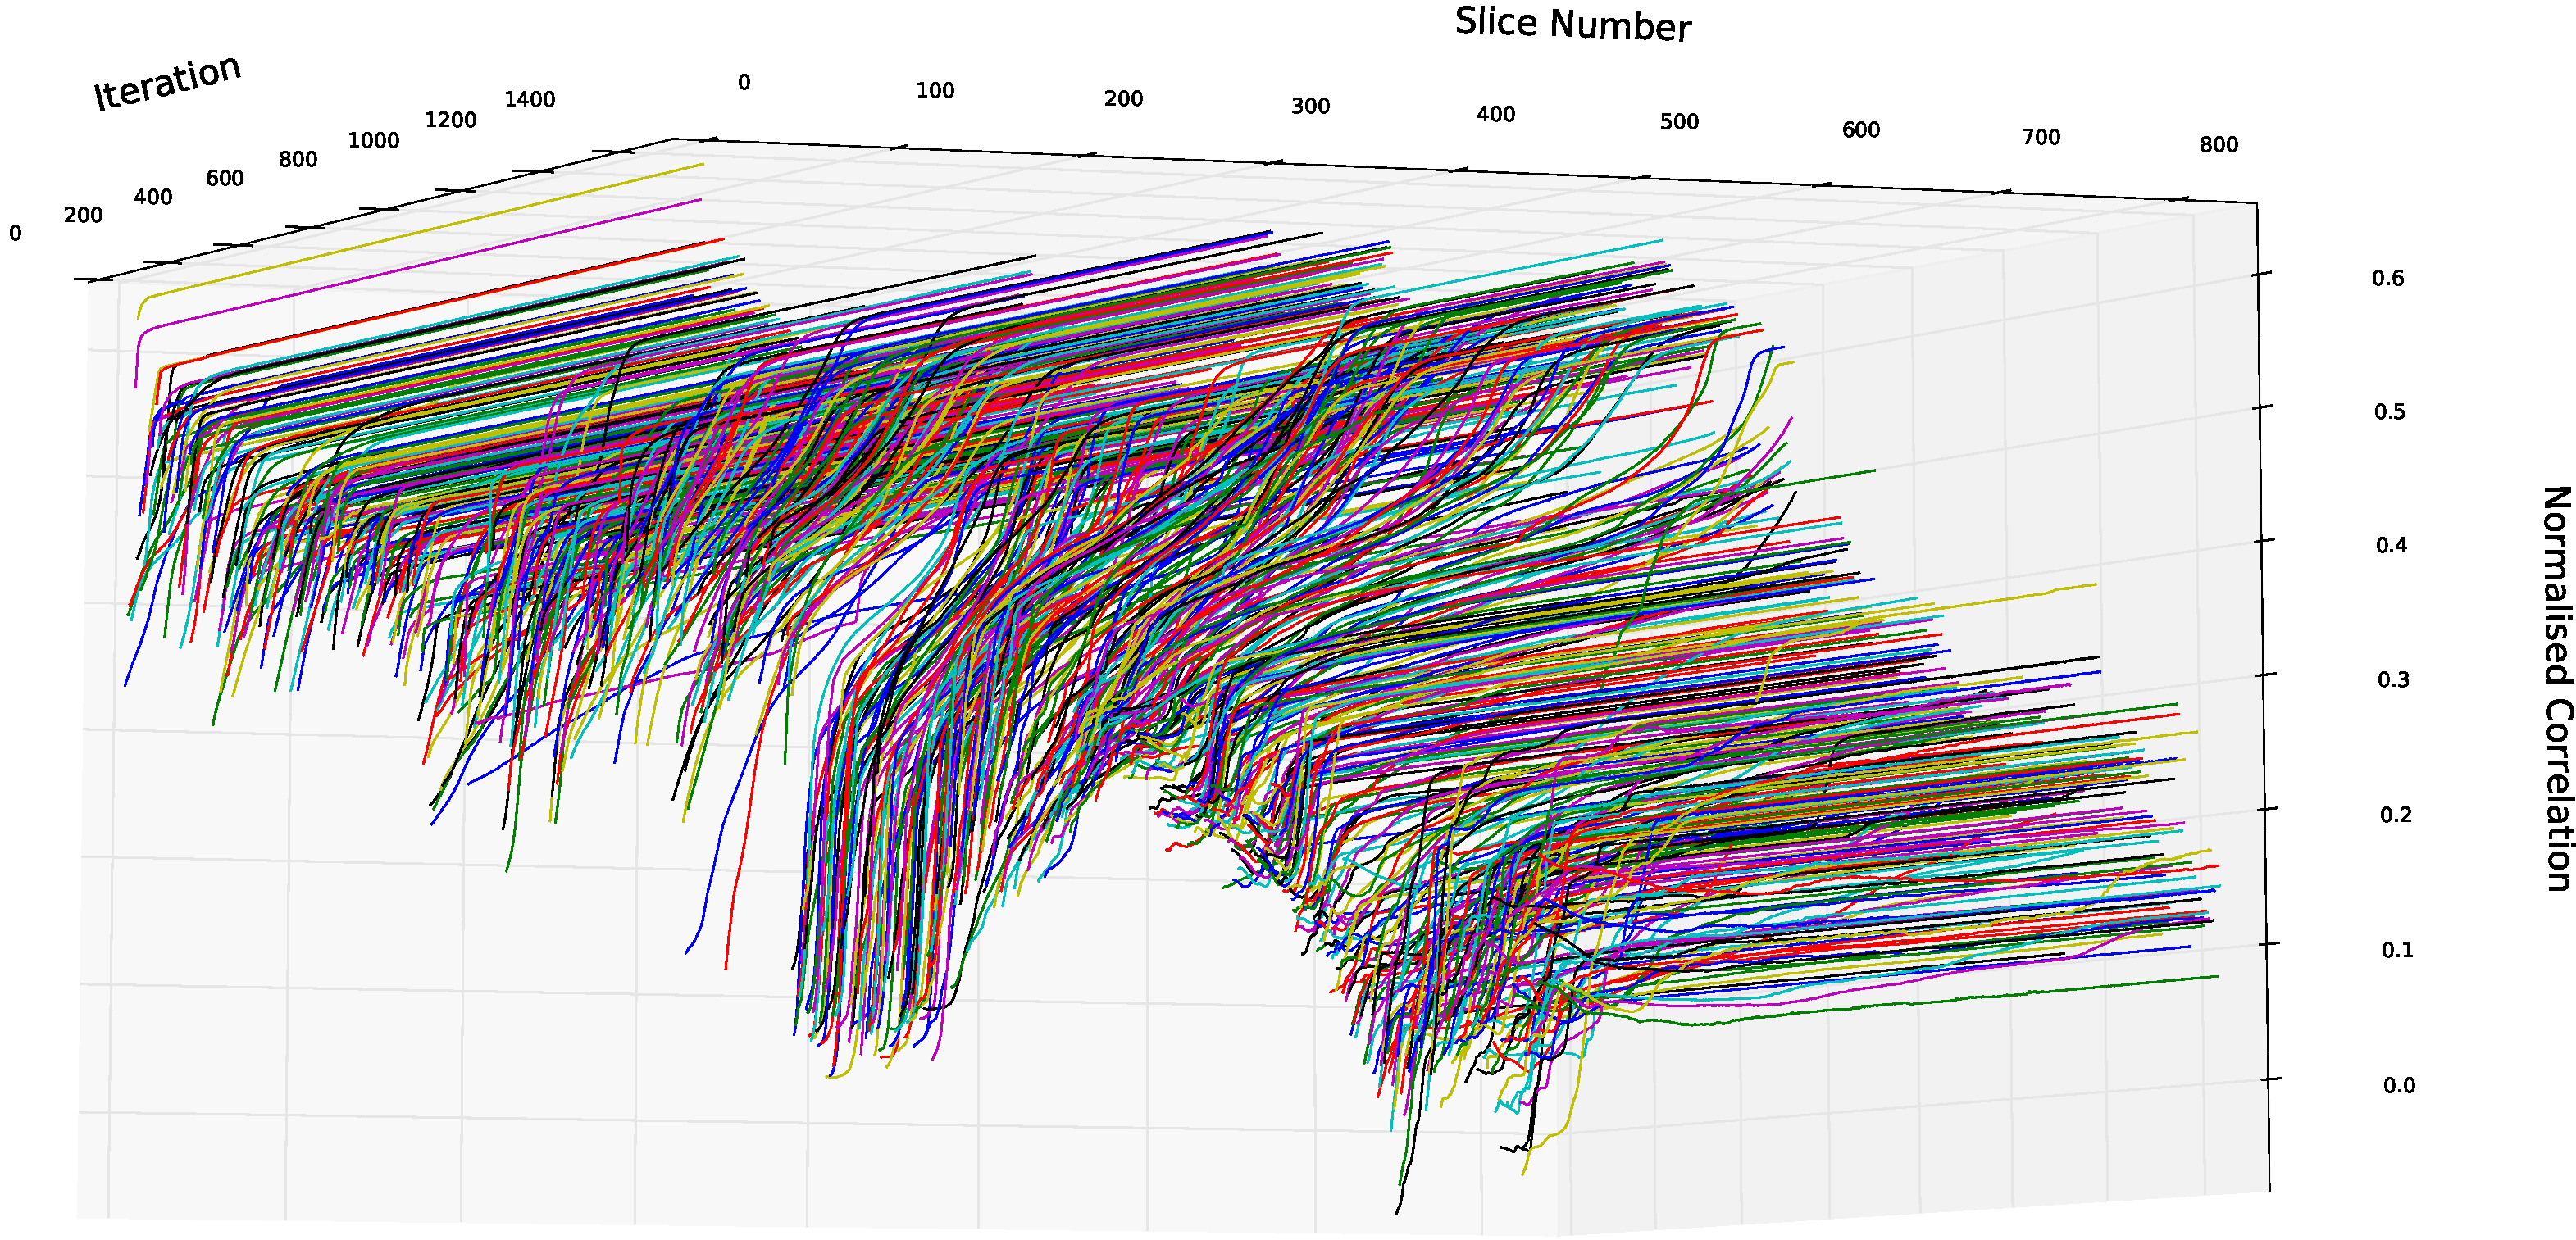
\includegraphics[width=\textheight]{Ch5/Figs/diagnostics/rigid_metric_values}
    \caption{Intermediate metric values for all slices during rigid registration.}
    \label{fig:rigid_metric_values}
  \end{sidewaysfigure}
      
  \begin{sidewaysfigure}[htbp]
    \centering
    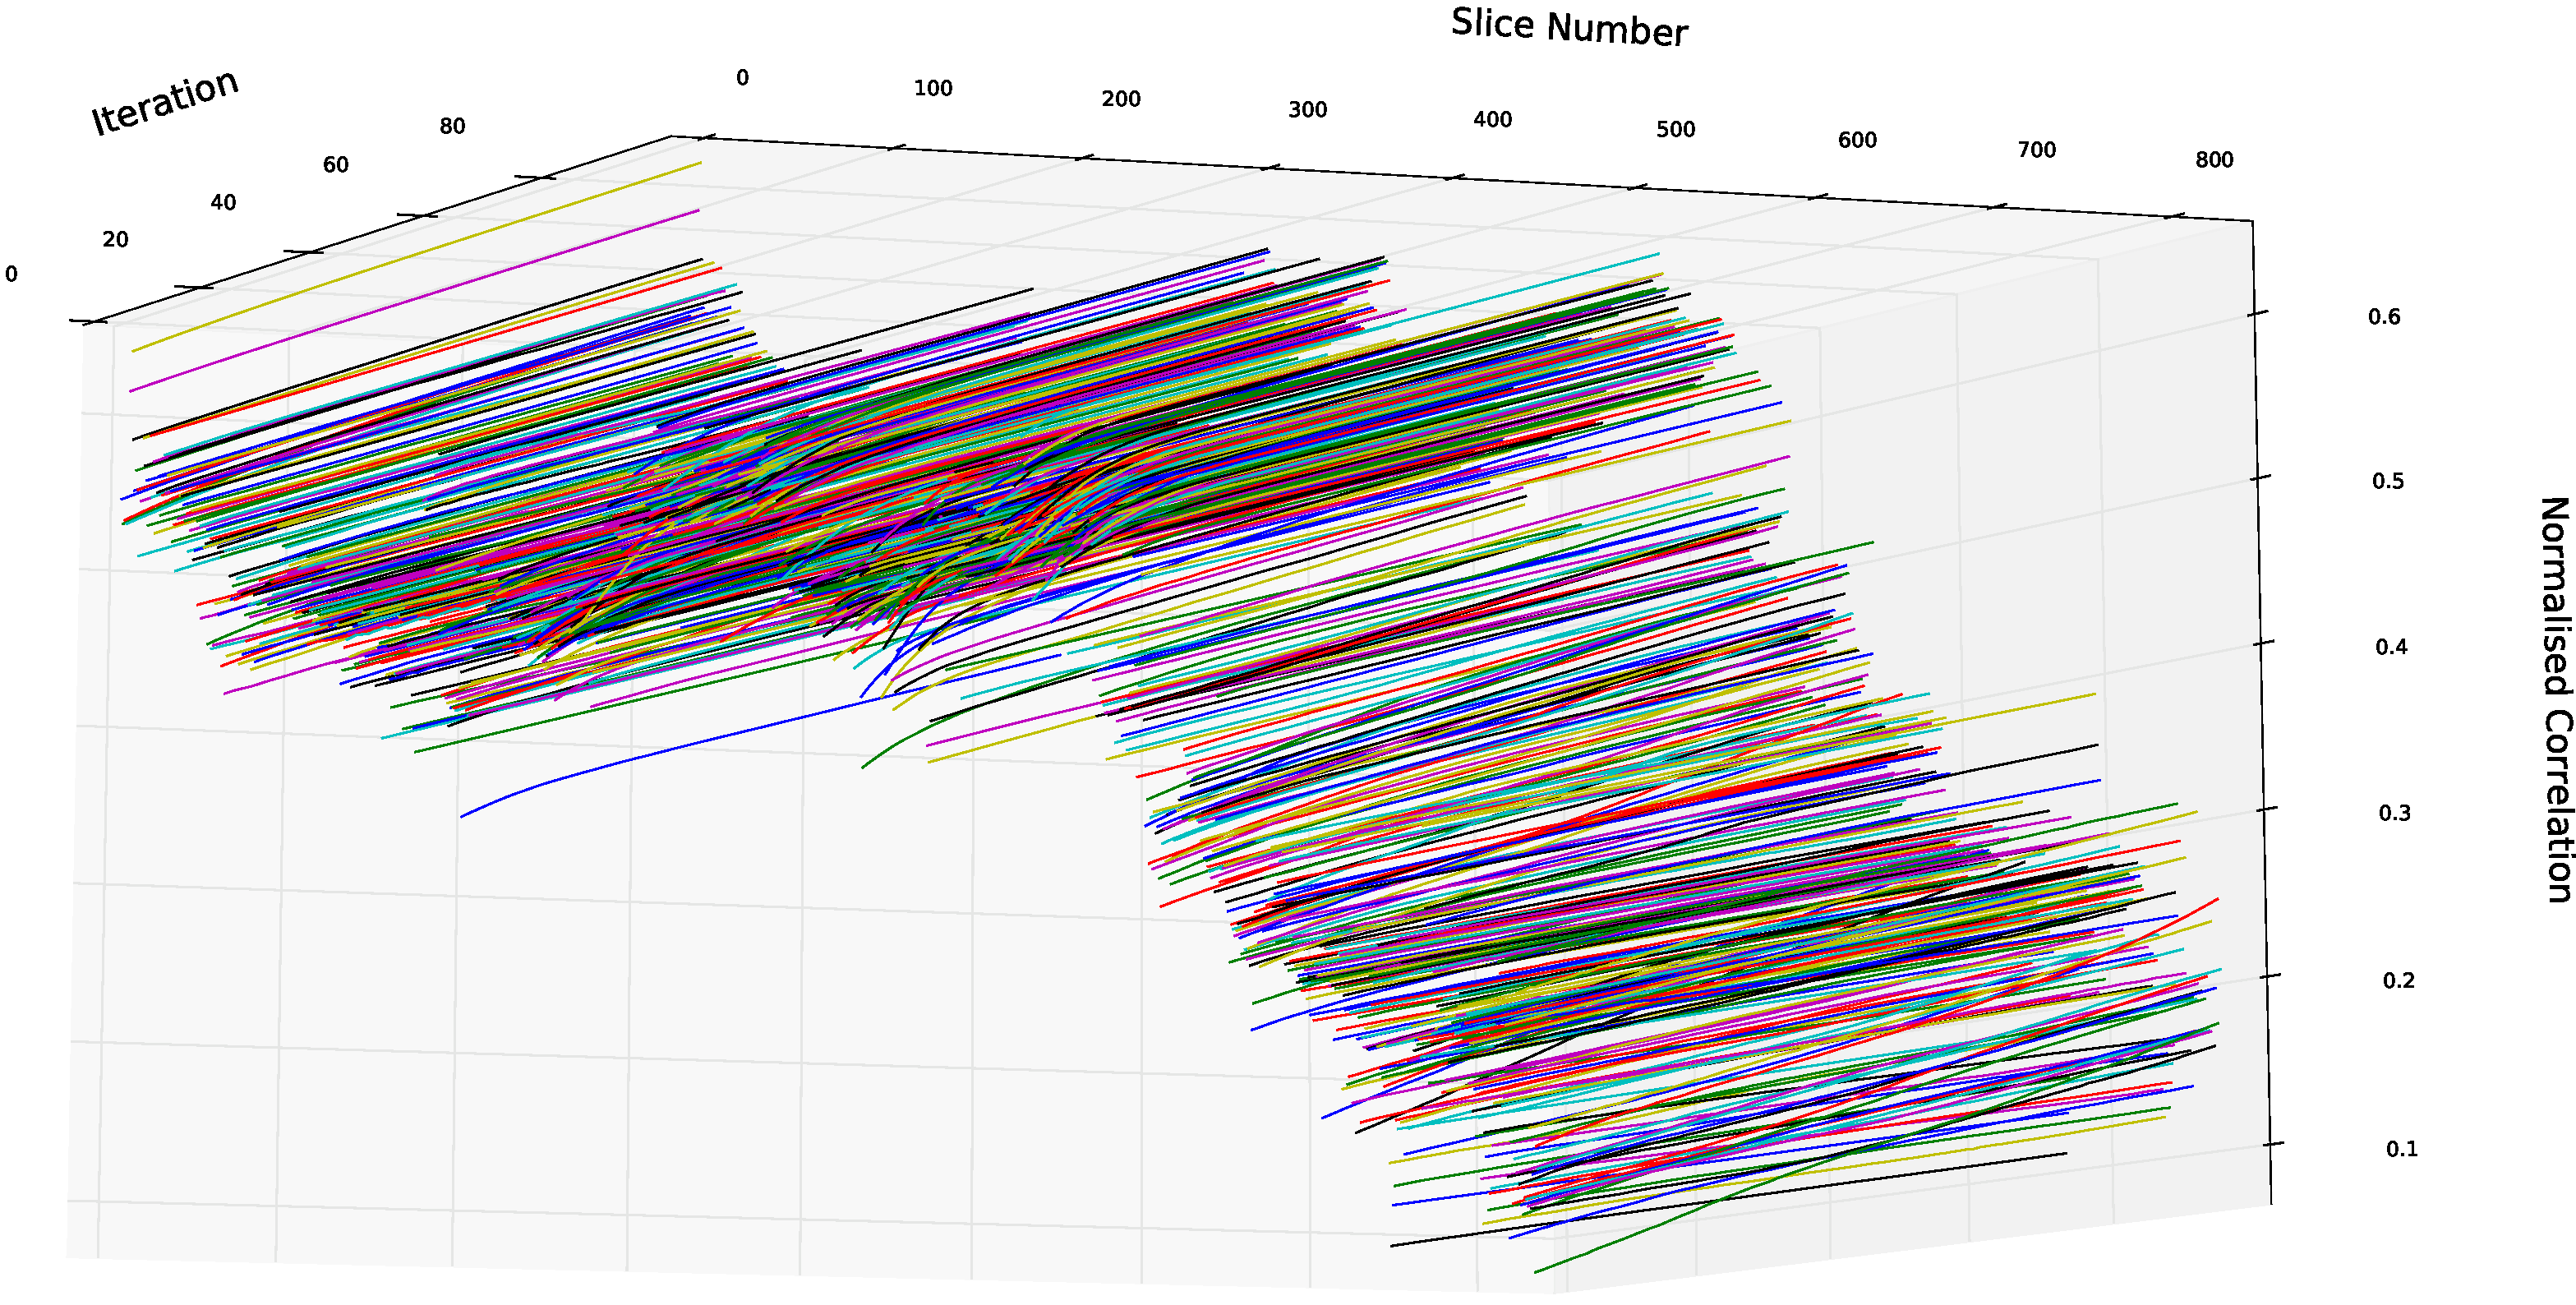
\includegraphics[width=\textheight]{Ch5/Figs/diagnostics/similarity_metric_values}
    \caption{Intermediate metric values for all slices during similarity registration.}
    \label{fig:similarity_metric_values}
  \end{sidewaysfigure}
      
  \begin{sidewaysfigure}[htbp]
    \centering
    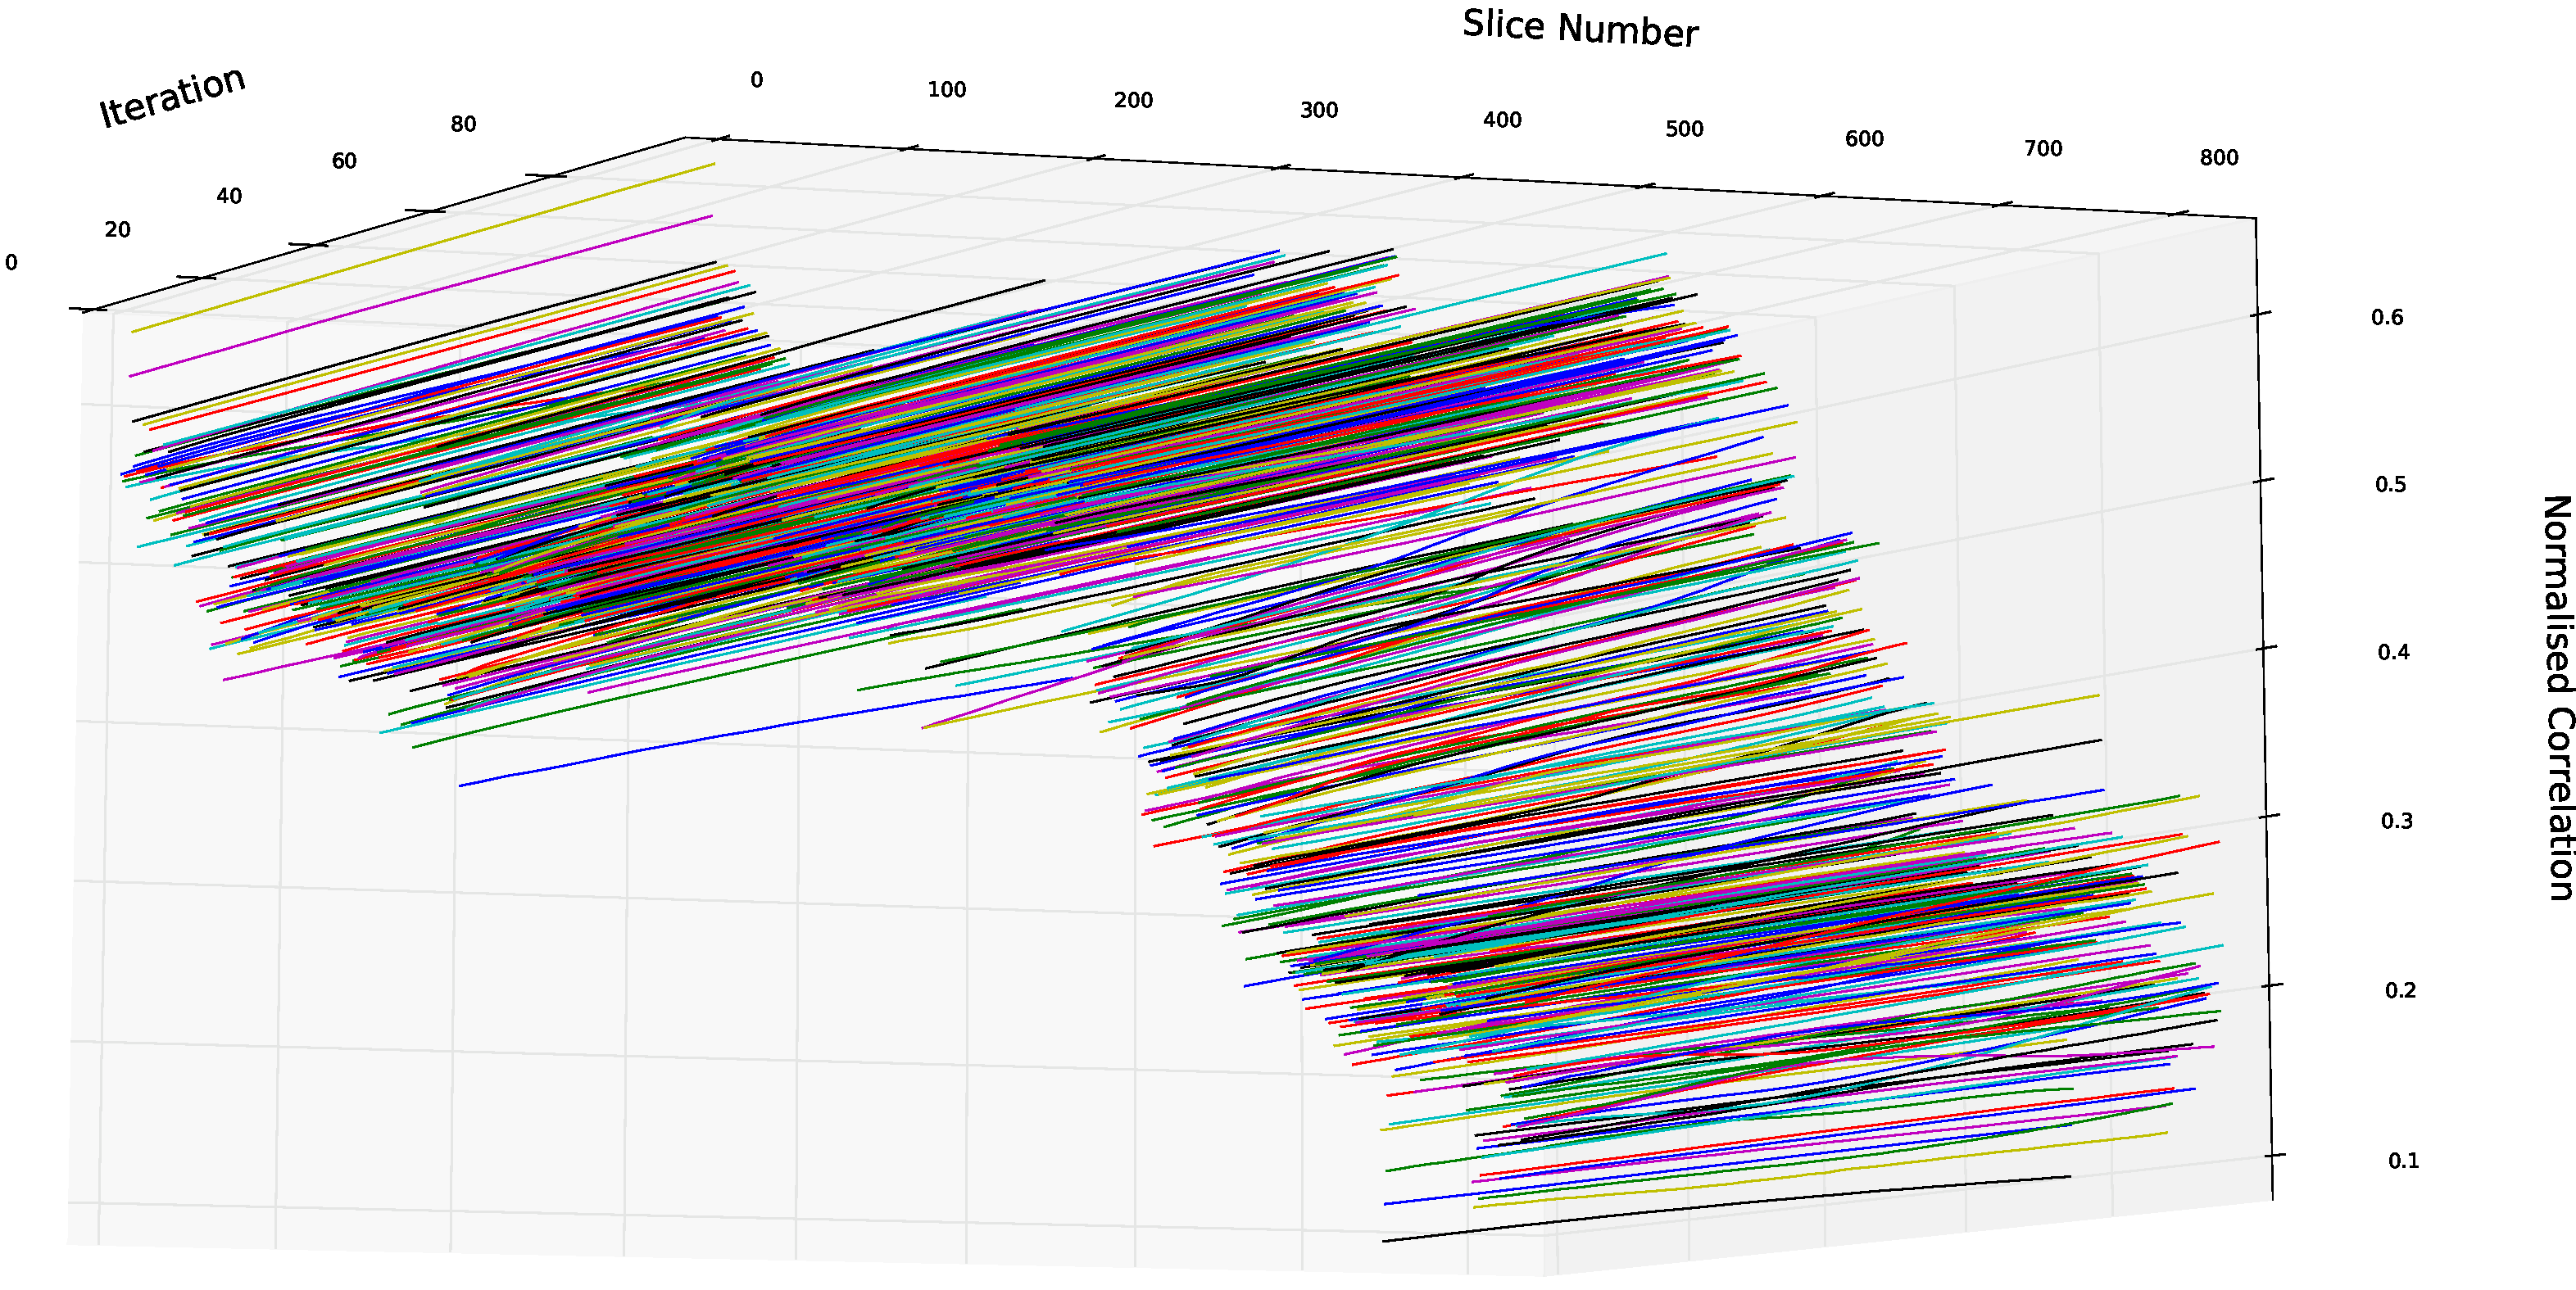
\includegraphics[width=\textheight]{Ch5/Figs/diagnostics/affine_metric_values}
    \caption{Intermediate metric values for all slices during affine registration.}
    \label{fig:affine_metric_values}
  \end{sidewaysfigure}
  
	Figures~\labelcref{fig:rigid_metric_values,fig:similarity_metric_values,fig:affine_metric_values} graph the intermediate metric values of each iteration for each slice, during the rigid, similarity and affine registrations. Each graph is viewed from below, in order to see all values clearly. Evidently, the overwhelming majority of the optimisation is done in the first rigid step, and this is reflected in the number of iterations required to reach a global optimum: 1500, as apposed to 100 for similarity and affine registrations. Nearly all curves increase smoothly and monotonically, before reaching a distinct flat maximum. In Figure~\ref{fig:rigid_metric_values} after around slice 600, where the blob-shaped artefact appears, the final metric values decrease almost linearly as the intensity of the blob increases. Slices in the region of 400-600 start from a much lower metric value, and take up to 1500 iterations to maximise; their geometric initialisations were much further from their final optimal position. Diagnostics were of critical importance here, not least to ensure that enough iterations had passed so that all slices had reached their flat optimum position.
	
  \begin{sidewaysfigure}[htbp]
    \centering
    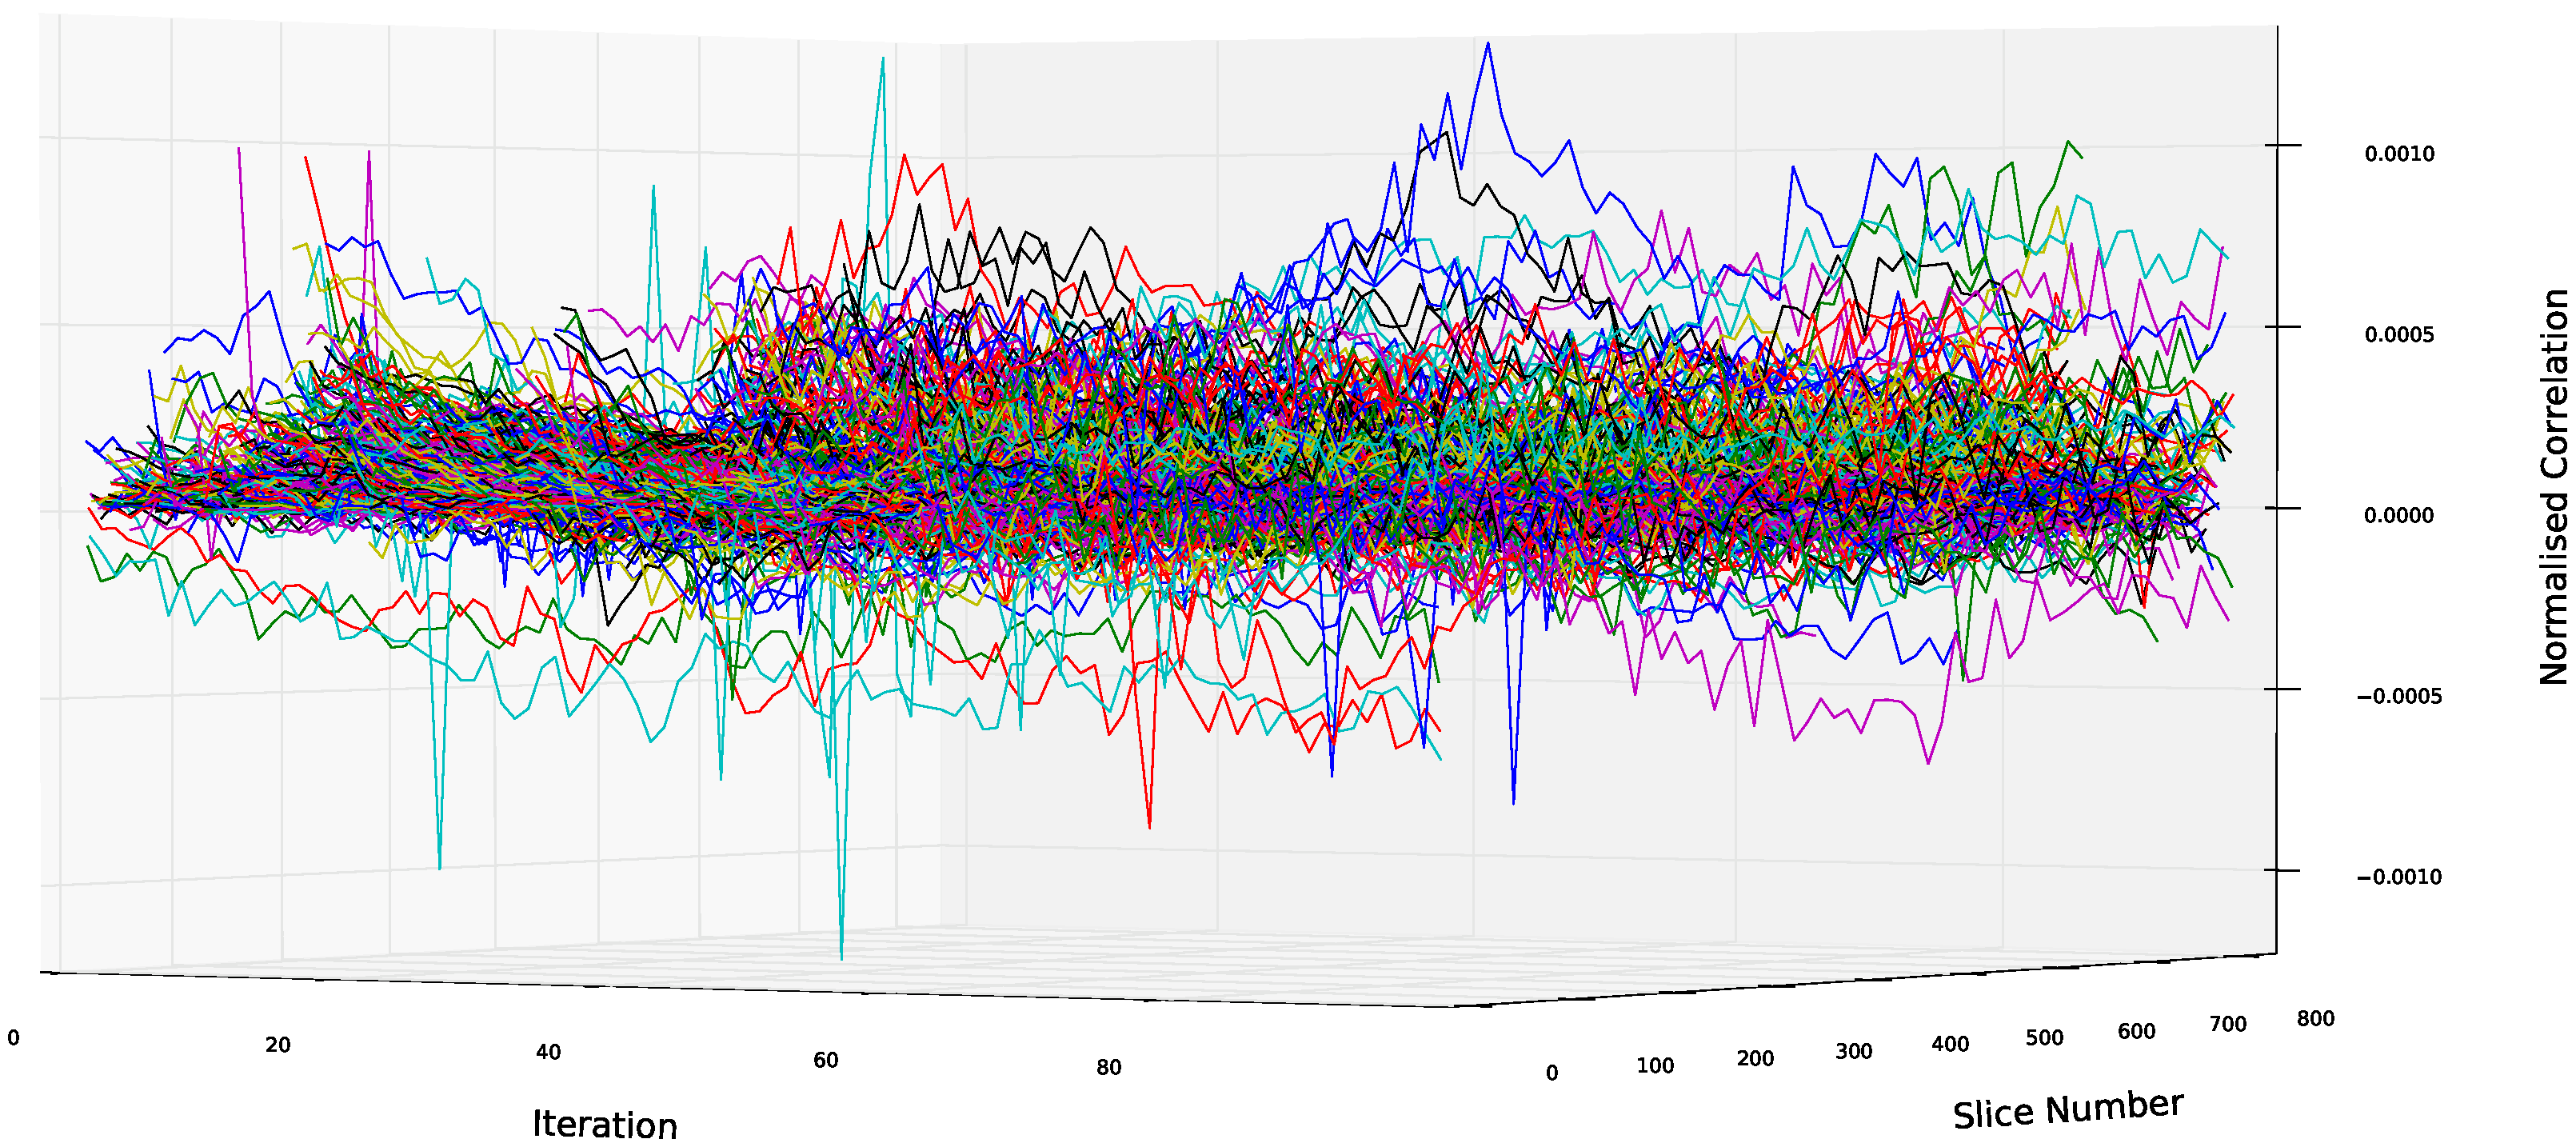
\includegraphics[width=\textheight]{Ch5/Figs/diagnostics/affine_metric_value_differences}
    \caption{Intermediate \emph{delta} metric values for all slices during affine registration.}
    \label{fig:affine_metric_value_differences}
  \end{sidewaysfigure}
  
	The changes in metric value in Figure~\ref{fig:affine_metric_values} are very small compared to the range of metric values across slices. Figure~\ref{fig:affine_metric_value_differences} depicts the change in metric value upon each iteration. It is viewed from the zero plane, and demonstrates -- at least to some extent -- that these changes are weighted largely to the positive side of zero. The affine registration is a small but certain improvement upon the similarity registration.
	
  \begin{sidewaysfigure}[htbp]
    \centering
    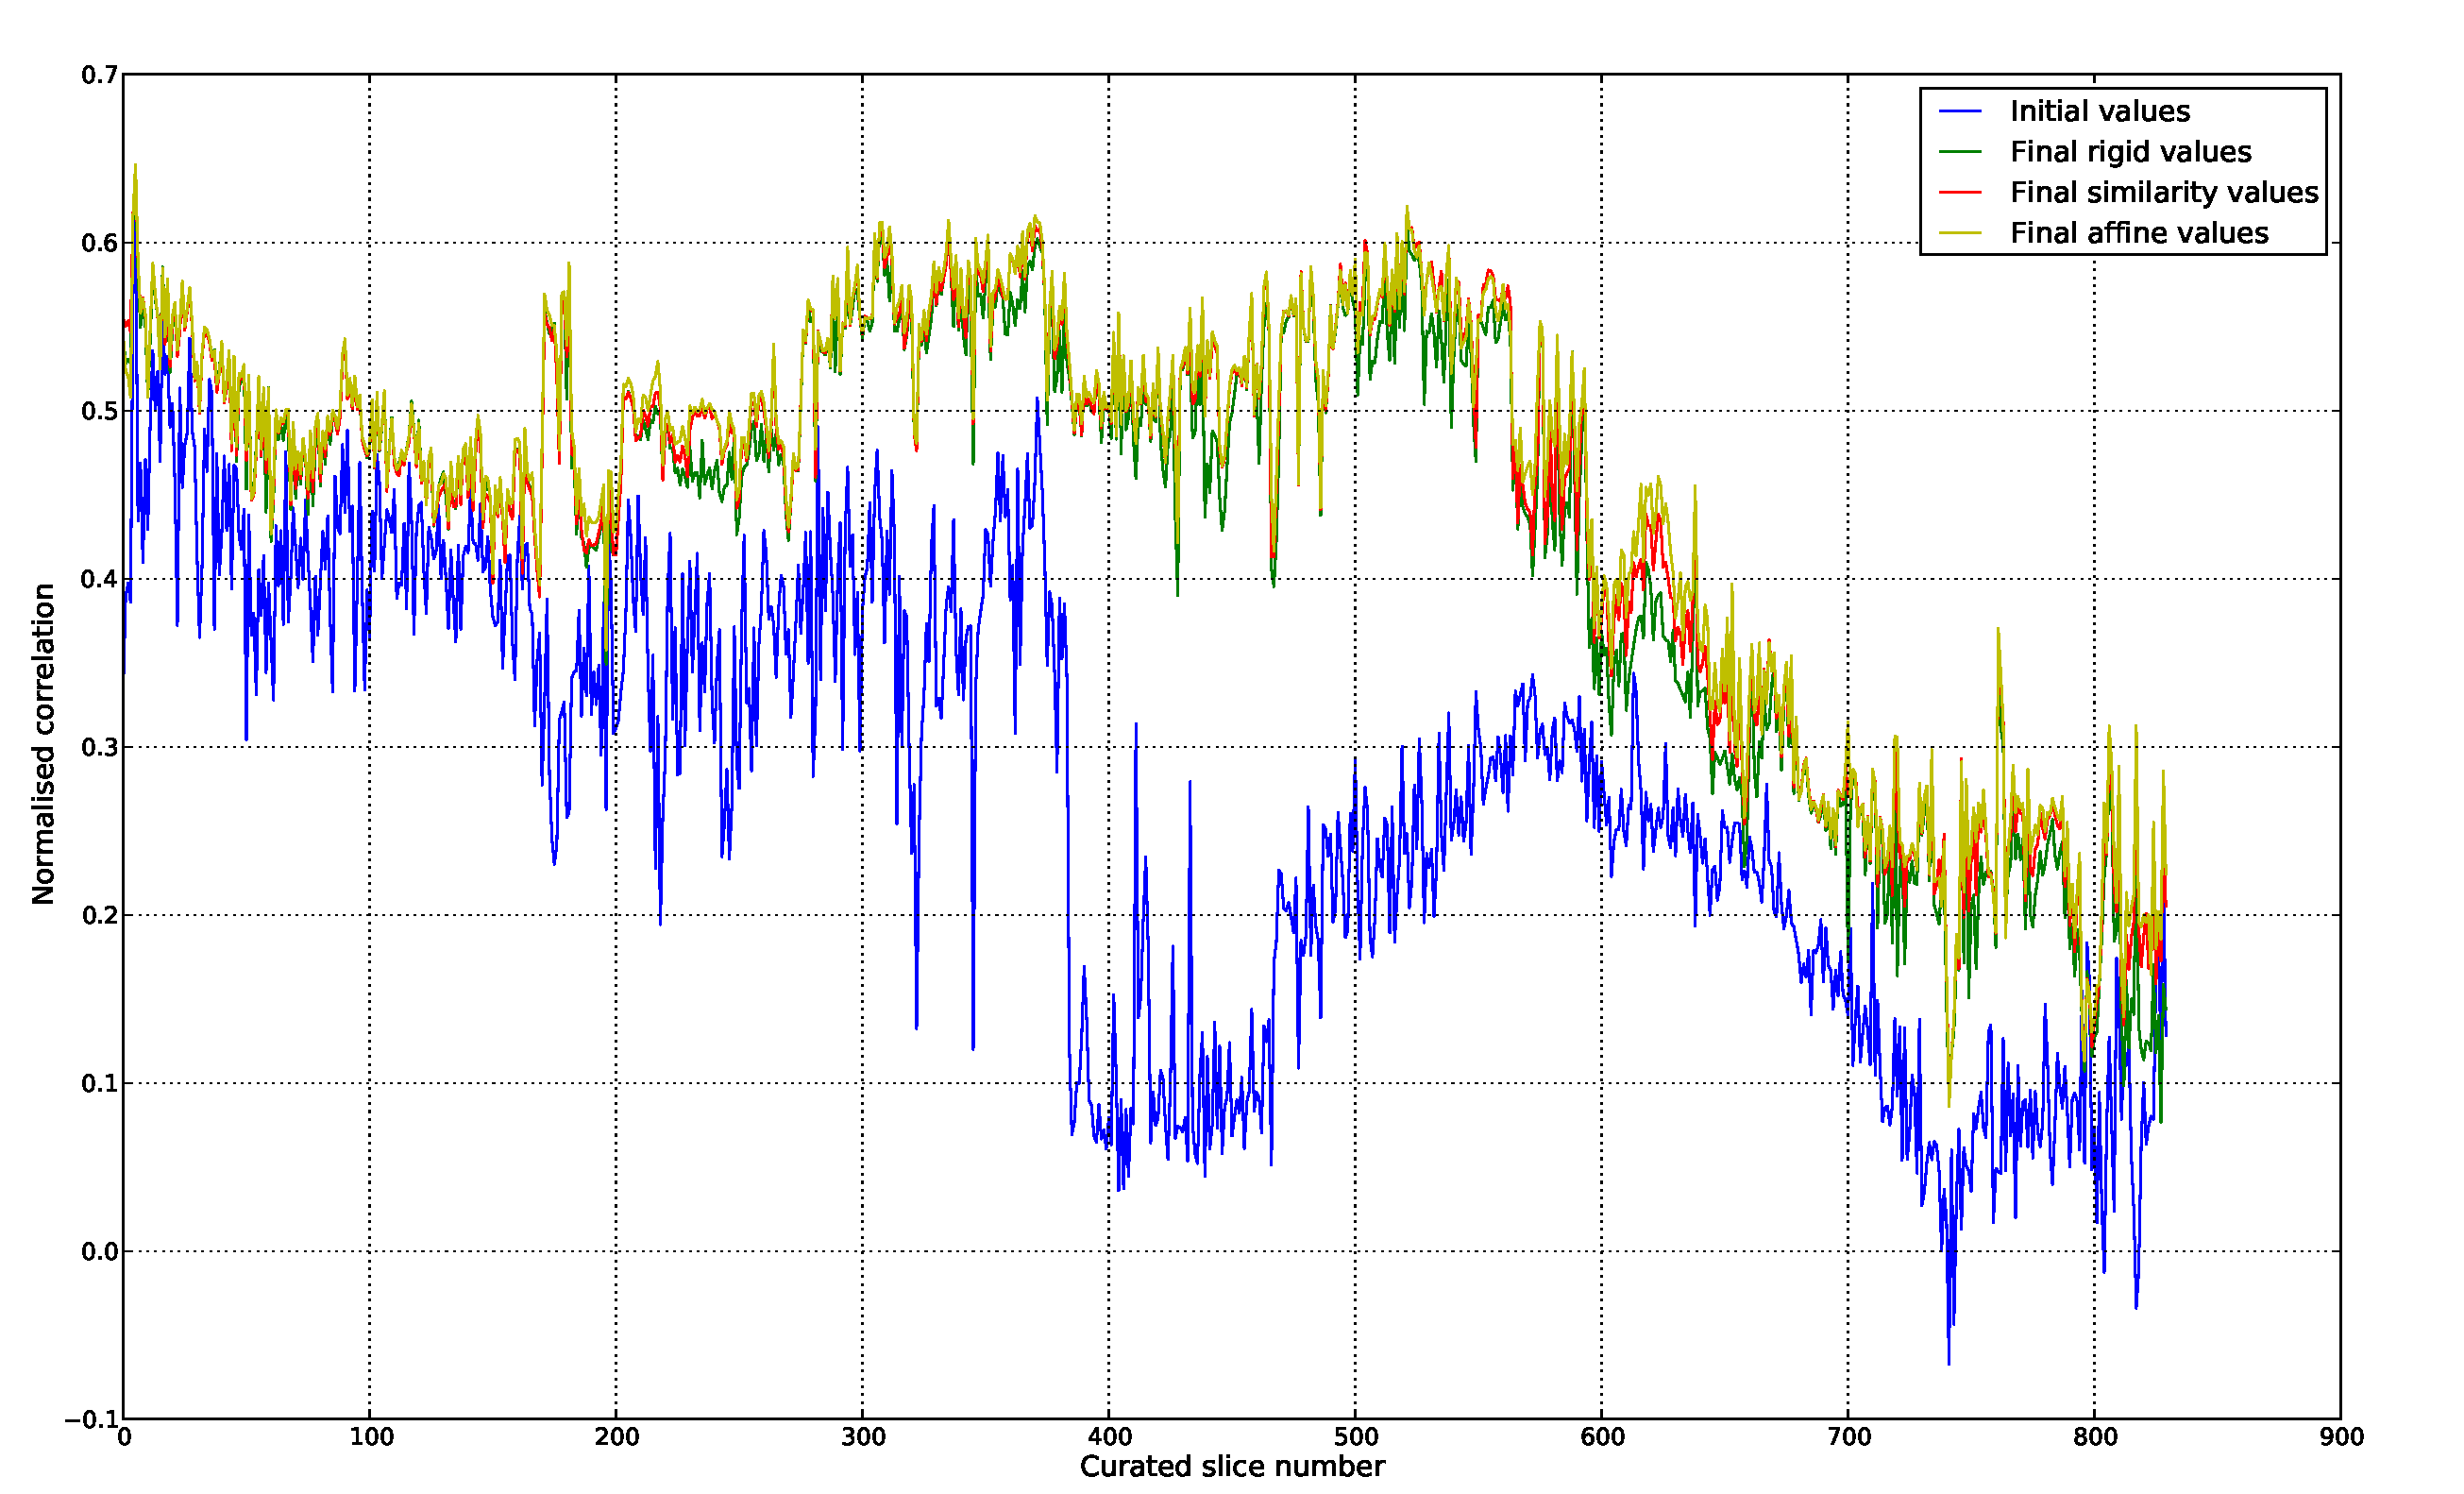
\includegraphics[width=\textheight]{Ch5/Figs/diagnostics/initial_and_final_values_comparison}
    \caption{Initial and final metric values before and after each stage of registration.}
    \label{fig:initial_and_final_values_comparison}
  \end{sidewaysfigure}
  
	Figure \ref{fig:initial_and_final_values_comparison} shows the initial metric values after geometric initialisation, and the final metric values after rigid, similarity and affine registrations. Again is it clear that each successive registration increases correlation, but the majority of improvement comes from the rigid registration. Slices from 380 to 600 were photographed at a larger angle from that of their block-face images, and this is reflected in a sharply reduced initial correlation value. From Slice 600 onwards, the blob precludes successful registration and both initial and final correlation values decline.
	
	\begin{figure}[htbp]
    \centering
    \subfigure[][]{
\includegraphics[height=0.3\textheight]{Ch5/Figs/diagnostics/fixed_progress_slice_0562_1_287.pdf}}
    \subfigure[][]{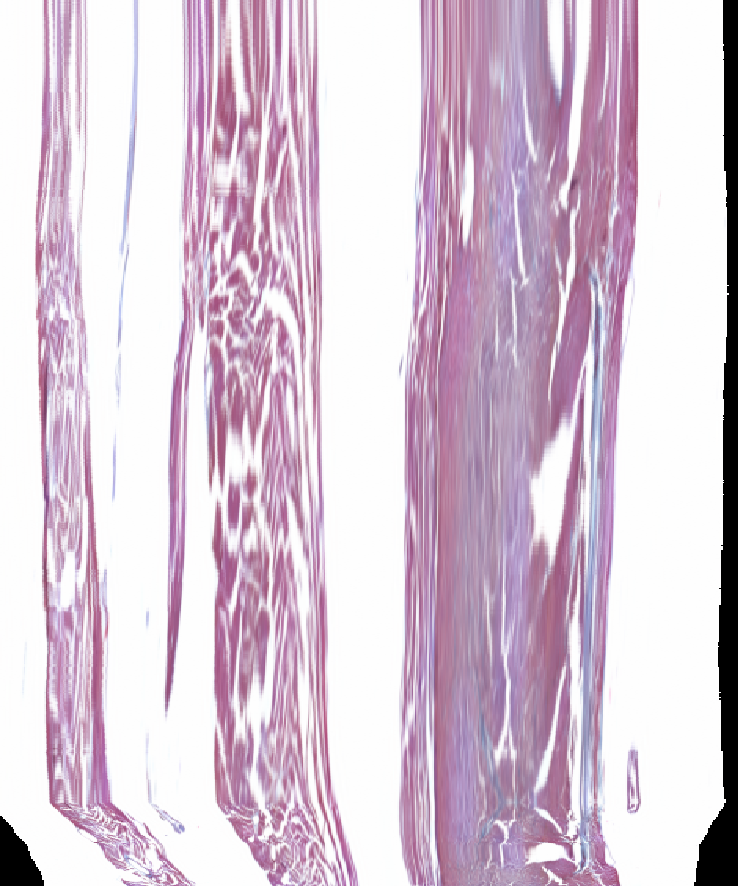
\includegraphics[height=0.3\textheight]{Ch5/Figs/diagnostics/moving_progress_slice_0562_1_287.pdf}}
    \subfigure[][]{
\includegraphics[height=0.3\textheight]{Ch5/Figs/diagnostics/fixed_progress_slice_0562_0_235.pdf}}
    \subfigure[][]{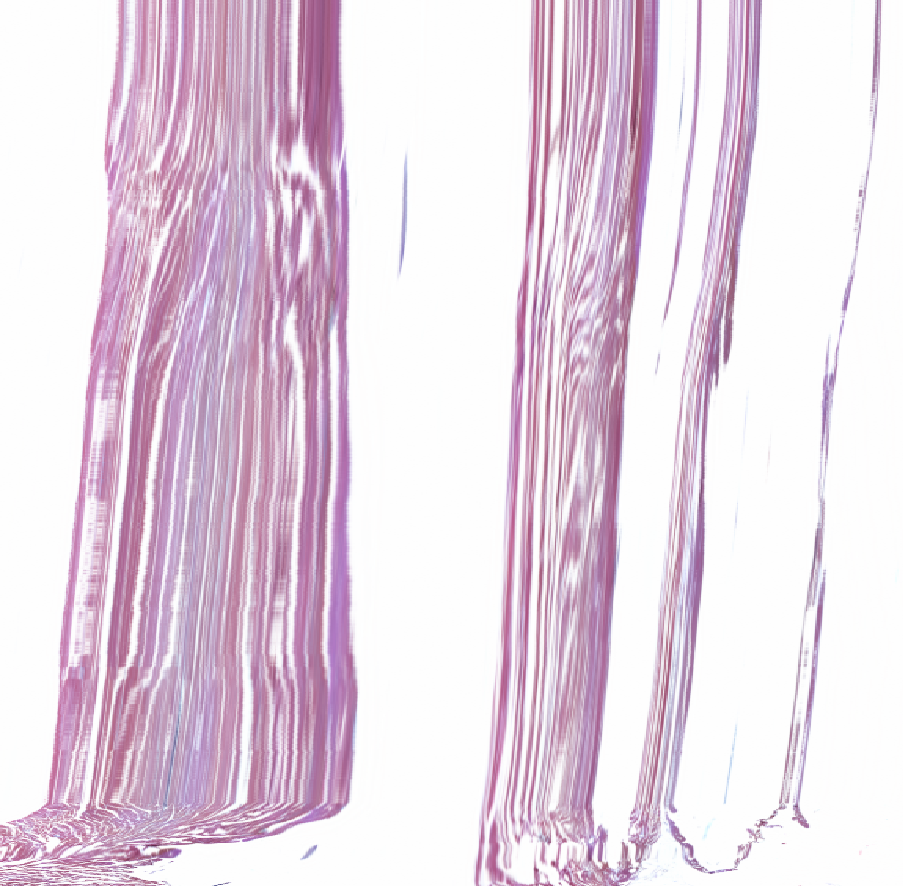
\includegraphics[height=0.3\textheight]{Ch5/Figs/diagnostics/moving_progress_slice_0562_0_235.pdf}}
    \caption{Central cross-sections of the progress volume of 1500 iterations of slice 0562, together with the fixed progress volume of the equivalent block face image.}
    \label{fig:progress_cross_sections}
  \end{figure}
      
  \begin{figure}[htbp]
    \centering
    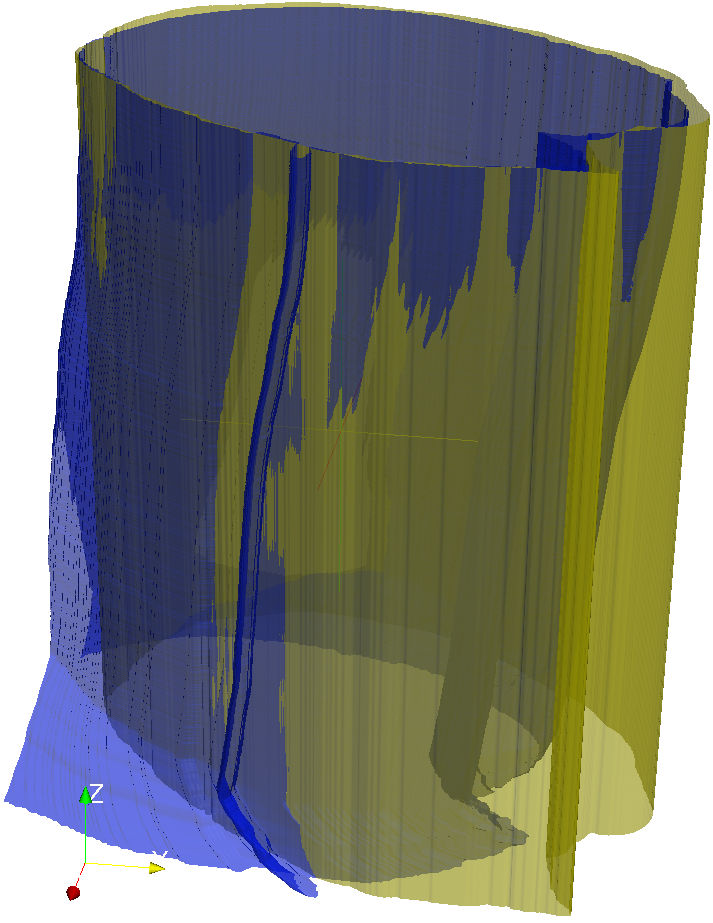
\includegraphics[width=\pagewidth]{Ch5/Figs/diagnostics/0562_contour.png}
    \caption{Contours of the progress volume of 1500 iterations of slice 0562 in blue, and of the fixed eqiuvalent block face image in yellow. Isosurfaces were extracted from volumes built from manual segmentations of both the block face and the slice image.}
    \label{fig:progress_contour}
  \end{figure}
      
  \begin{figure}[p]
    \centering
    \subfigure[][]{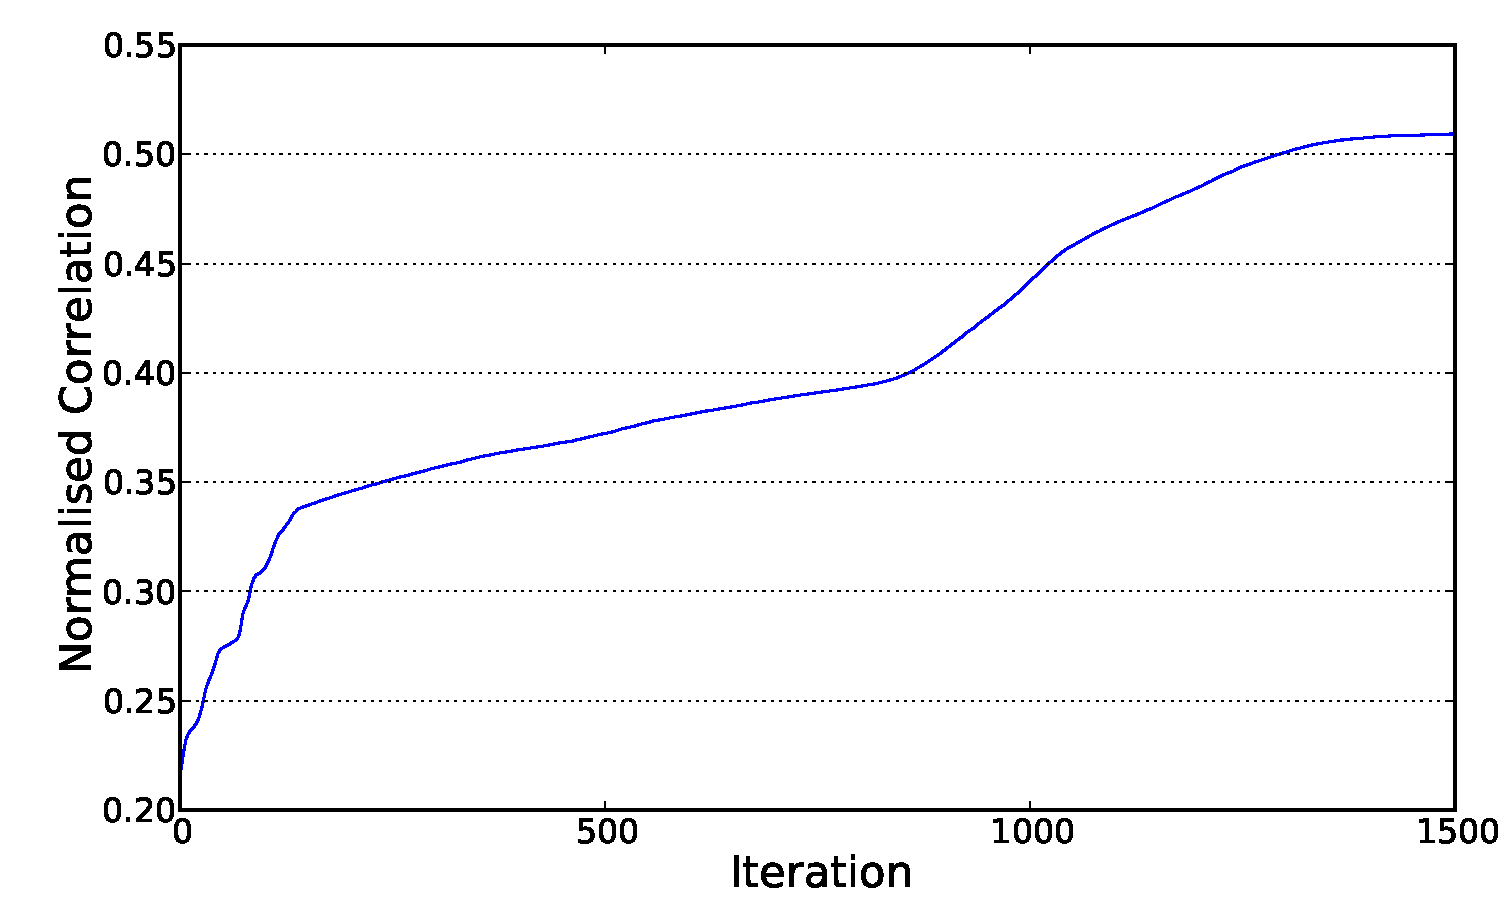
\includegraphics[width=0.9\pagewidth]{Ch5/Figs/diagnostics/0562_correlation}}
    \subfigure[][]{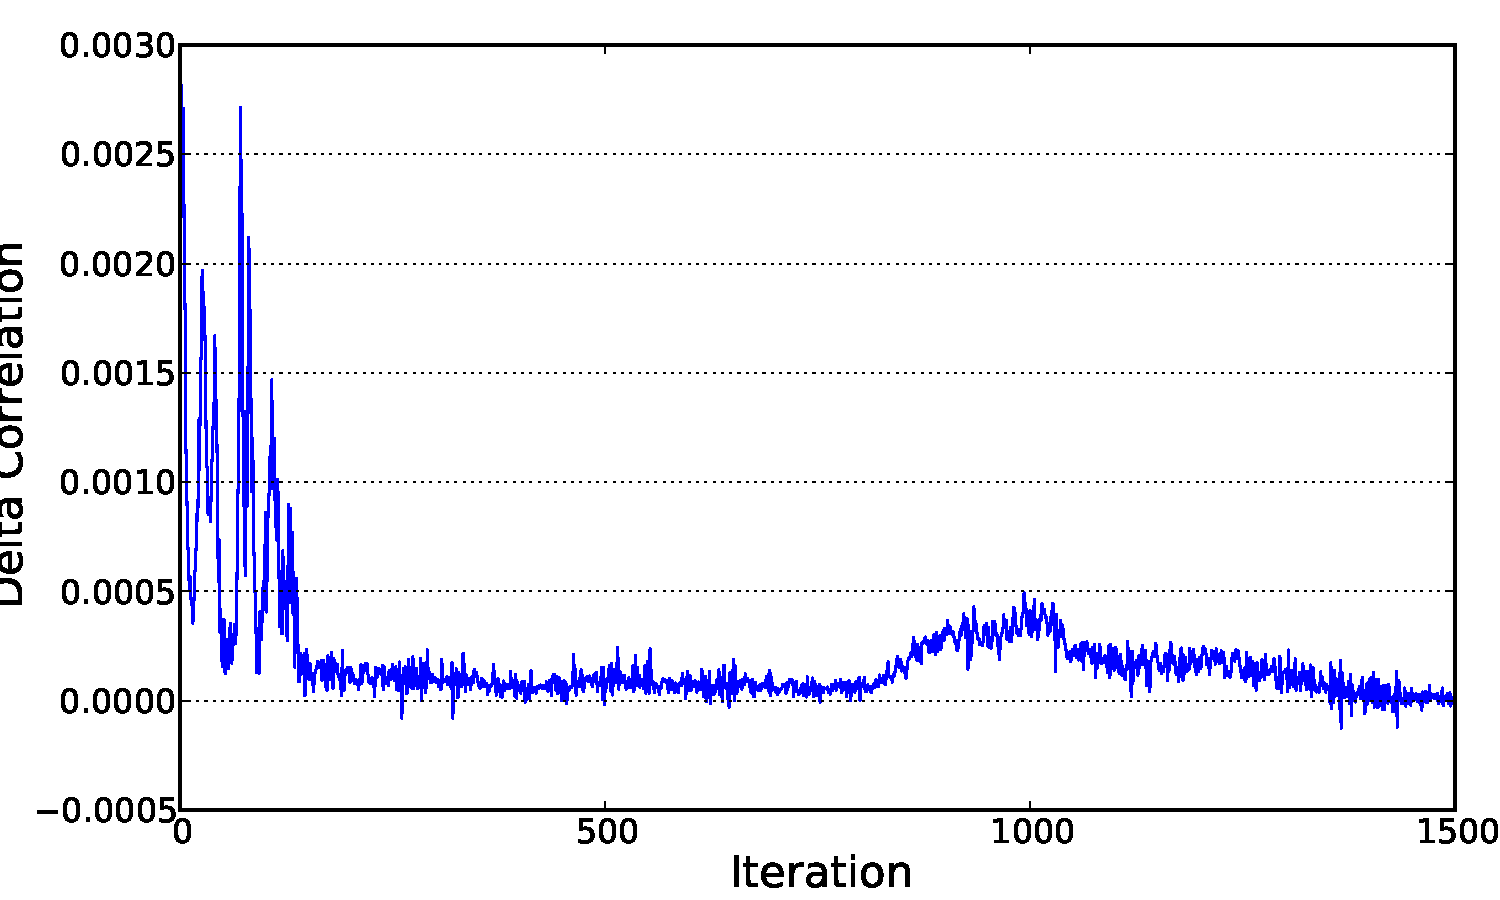
\includegraphics[width=0.9\pagewidth]{Ch5/Figs/diagnostics/0562_delta_correlation}}
    \caption{Metric values and delta metric values during the rigid registration of slice 0562.}
    \label{fig:0562_correlation}
  \end{figure}
	
	Figures~\labelcref{fig:progress_cross_sections,fig:progress_contour,fig:0562_correlation} showcase the diagnostics for a single representative slice during rigid registration. Figures~\labelcref{fig:progress_cross_sections,fig:progress_contour} are representations of the progress volume: a stack of the same 0562 image, transformed by the updating rigid transform at each of the 1500 steps in the registration. The rotation angle is quickly optimised in the first 100 iterations at the base. A flatter, slower translational optimisation ensues, which finally reaches a stationary minimum over the last iterations at the top. The top of Figure~\ref{fig:progress_contour} shows a very close fit compared with the starting point. The distinct phases of the registration are mirrored in the metric values of Figure~\ref{fig:0562_correlation}. The rapid rotational phase is seen again in the first 100 steps, with the largest metric gradients of the whole registration. A smooth, monotonic translational phase for the next 700 iterations accelerates as it gets close to the optimum, until coming to rest at around 1450 iterations.
	
	% initialisation figure
	\begin{sidewaysfigure}[htbp]
	  \centering
	  \subfigure[][]{
\includegraphics[height=0.31\textheight]{Ch5/Figs/geometric_0_235}}
	  \subfigure[][]{
\includegraphics[height=0.31\textheight]{Ch5/Figs/geometric_1_287}}
	  \caption{Central cross-sections of the slice image stack before registration. \textbf{(a)} is perpendicular to the x-axis, and \textbf{(b)} to the y-axis.}
	  \label{fig:geometric_initialisation}
	\end{sidewaysfigure}

	% x slices
	\begin{figure}[htbp]
	  \centering
	  \subfigure[][]{
\includegraphics[height=0.31\textheight]{Ch5/Figs/rigid_0_235}}
	  \subfigure[][]{
\includegraphics[height=0.31\textheight]{Ch5/Figs/size_0_235}}
	  \subfigure[][]{
\includegraphics[height=0.31\textheight]{Ch5/Figs/affine_0_235}}
	  \caption{Cross-sections of the rigid, similarity and affine volumes perpendicular to the x-axis.}
	  \label{fig:hires_0_235}
	\end{figure}

	% y slices
	\begin{figure}[htbp]
	  \centering
	  \subfigure[][]{
\includegraphics[height=0.31\textheight]{Ch5/Figs/rigid_1_287}}
	  \subfigure[][]{
\includegraphics[height=0.31\textheight]{Ch5/Figs/size_1_287}}
	  \subfigure[][]{
\includegraphics[height=0.31\textheight]{Ch5/Figs/affine_1_287}}
	  \caption{Cross-sections of the rigid, similarity and affine volumes perpendicular to the y-axis.}
	  \label{fig:hires_1_287}
	\end{figure}

	Central cross-sections of the geometrically initialised volume before registration are shown in Figure~\ref{fig:geometric_initialisation}, and cross-sections after each stage of the registration are shown in Figures~\labelcref{fig:hires_0_235,fig:hires_1_287}. The incoherent volumes in Figure~\ref{fig:geometric_initialisation} are brought into alignment by rigid registration, with small incremental improvements from similarity and affine. The improvements in the later stages are most evident at the extremeties to the left and right of the figures, where the effects of small changes in parameters are most evident; edges are smoother, tissue microstructure is more clearly discerned and large displacements are mostly removed. Discontinuities in intensity between block face images, visible in Figure~\ref{fig:LoRes_cross_sections}, are mirrored in the registration. It is also clear that registration has failed from slice 600 upwards.
	
	% geometric contours
	\begin{sidewaysfigure}[p]
	  \centering
	  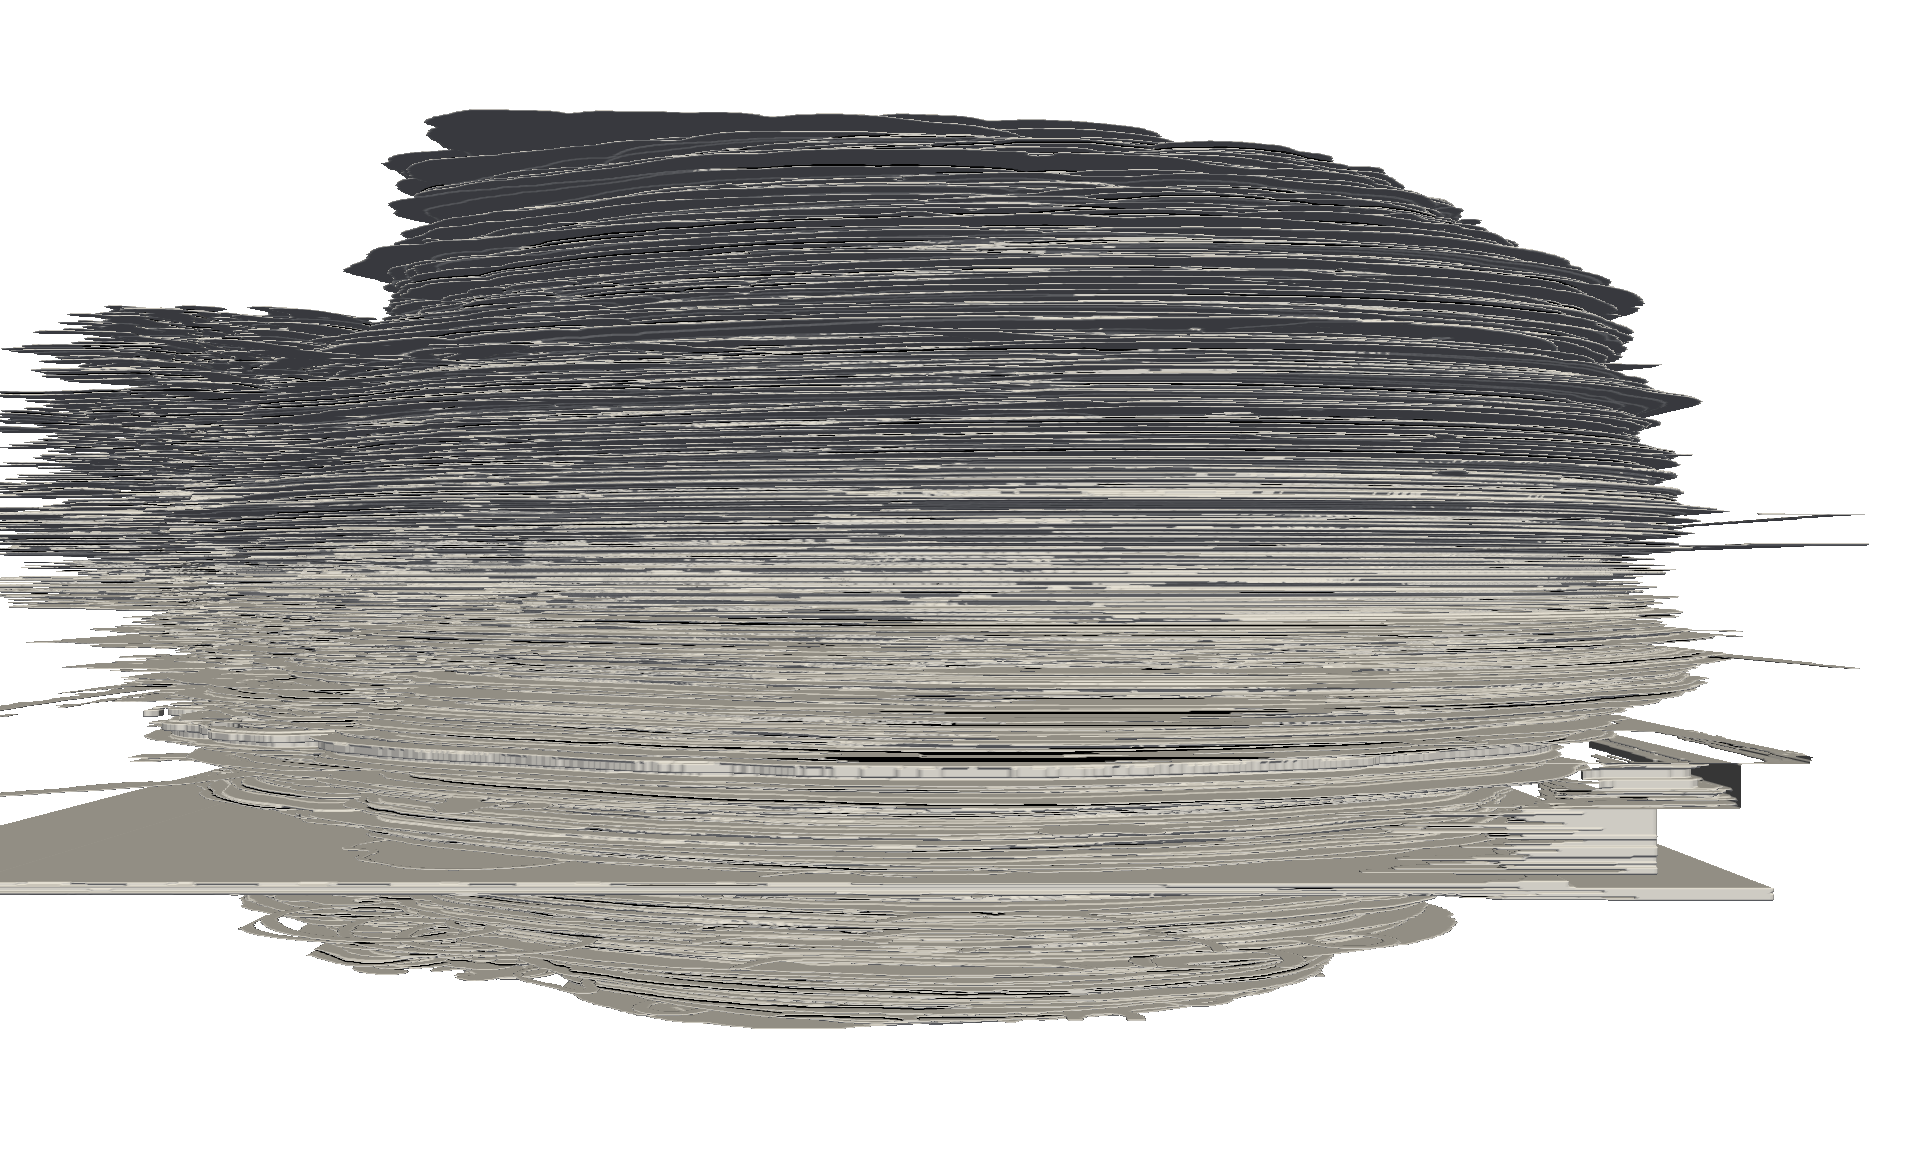
\includegraphics[width=0.9\textheight]{Ch6/Figs/Rat28/contours/whole_positive_x_geometric}
	  \caption{Geometric slice volume, viewed along the positive x direction.}
	  \label{fig:positive_x_geometric_contour}
	\end{sidewaysfigure}

	\begin{sidewaysfigure}[p]
	  \centering
	  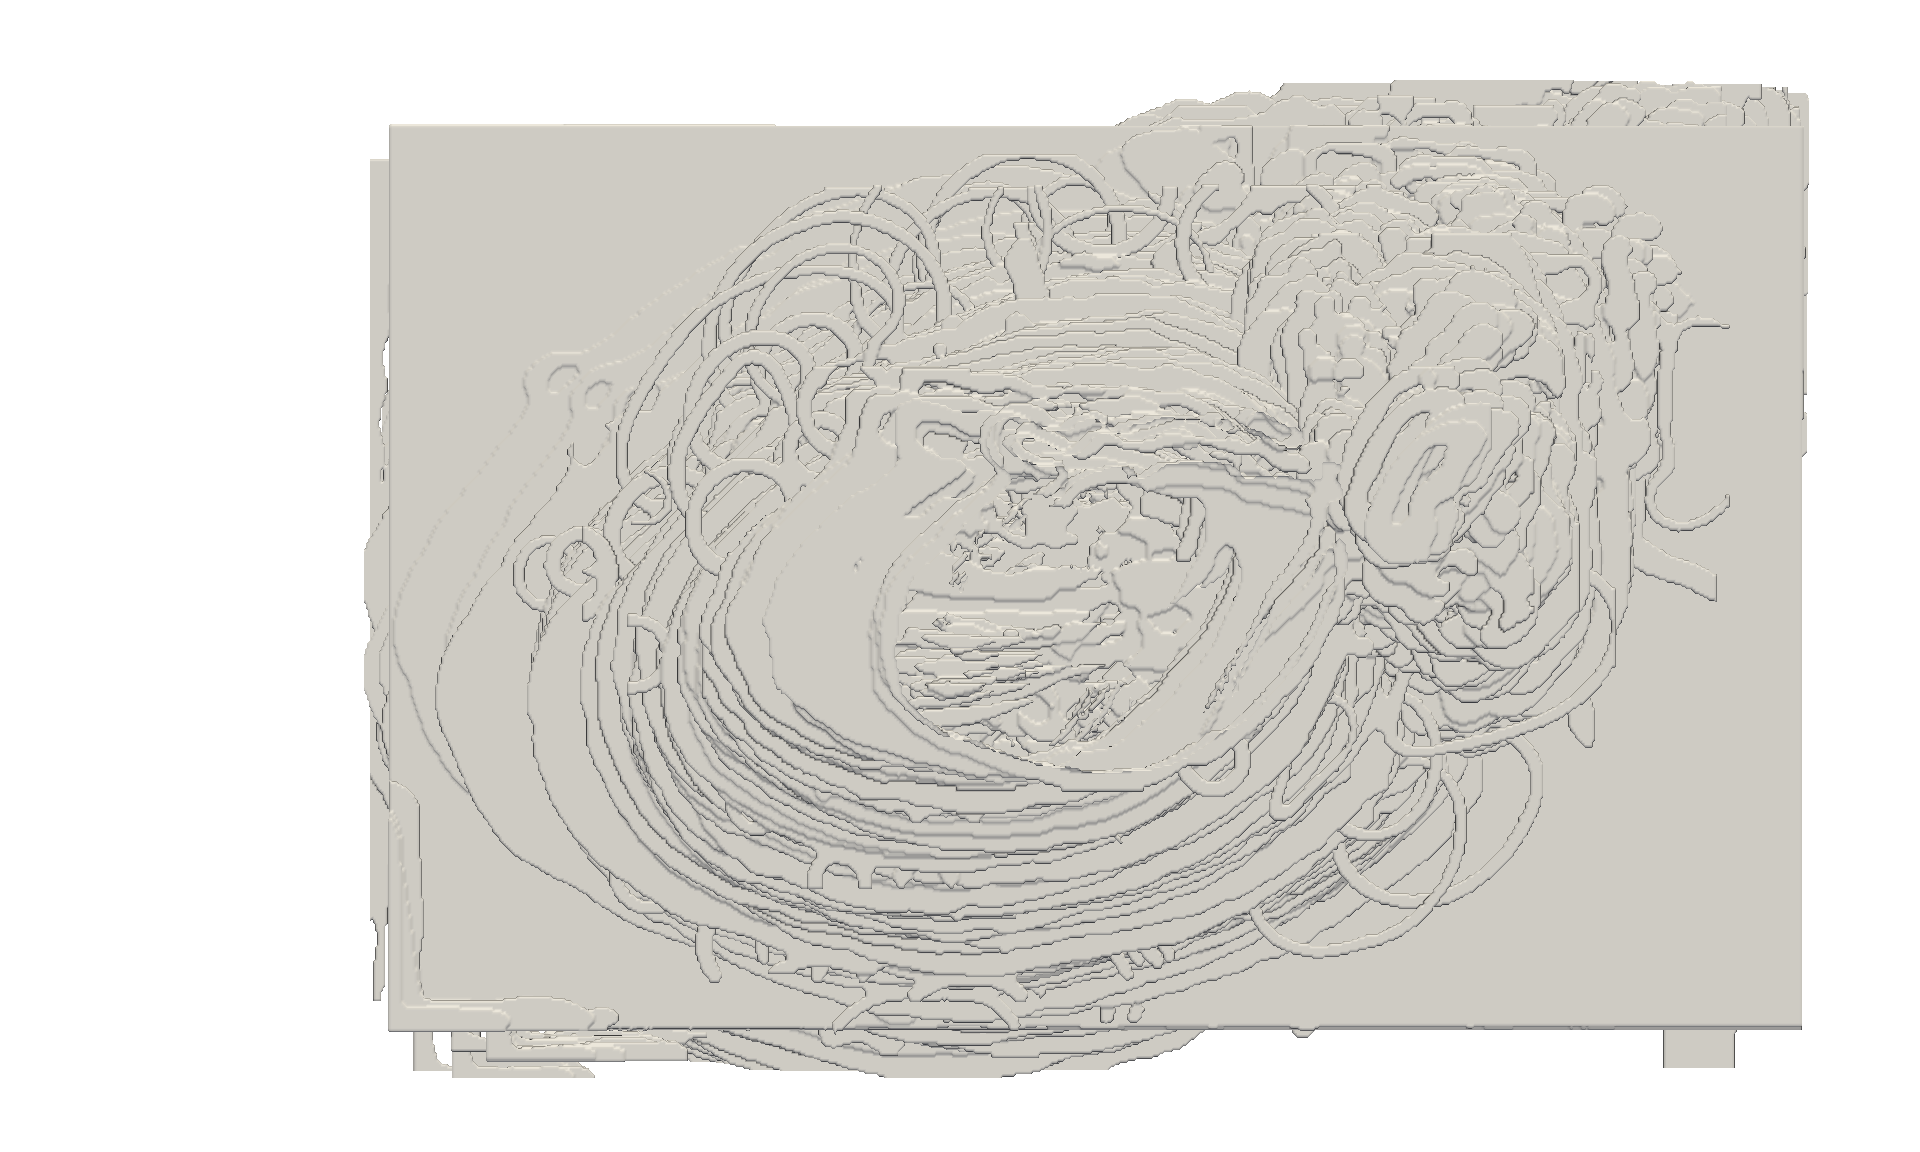
\includegraphics[width=0.9\textheight]{Ch6/Figs/Rat28/contours/whole_positive_z_geometric}
	  \caption{Geometric slice volume, viewed along the positive z direction.}
	  \label{fig:positive_z_geometric_contour}
	\end{sidewaysfigure}

	% affine contours
	\begin{sidewaysfigure}[p]
	  \centering
	  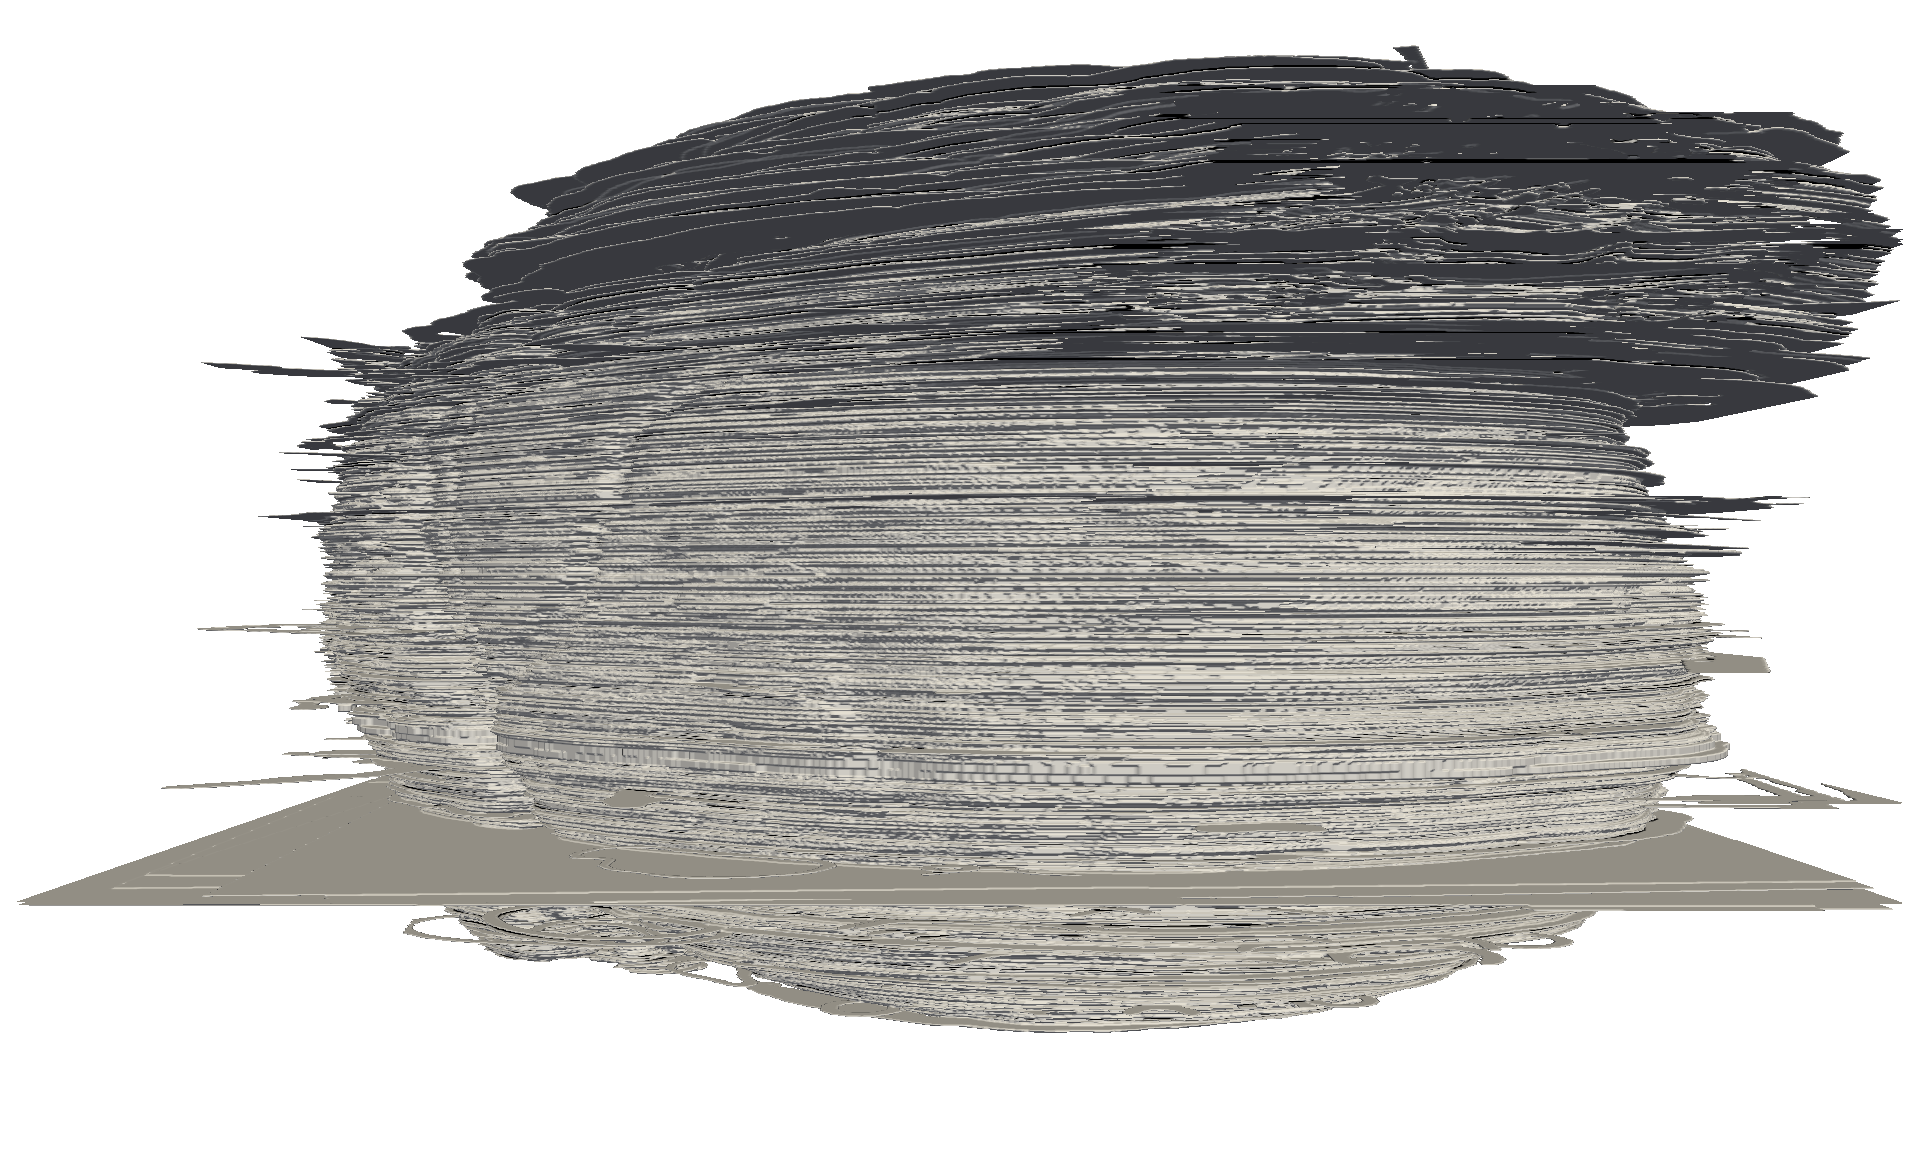
\includegraphics[width=0.9\textheight]{Ch6/Figs/Rat28/contours/whole_positive_x_affine}
	  \caption{Affine slice volume, viewed along the positive x direction.}
	  \label{fig:positive_x_affine_contour}
	\end{sidewaysfigure}

	\begin{sidewaysfigure}[p]
	  \centering
	  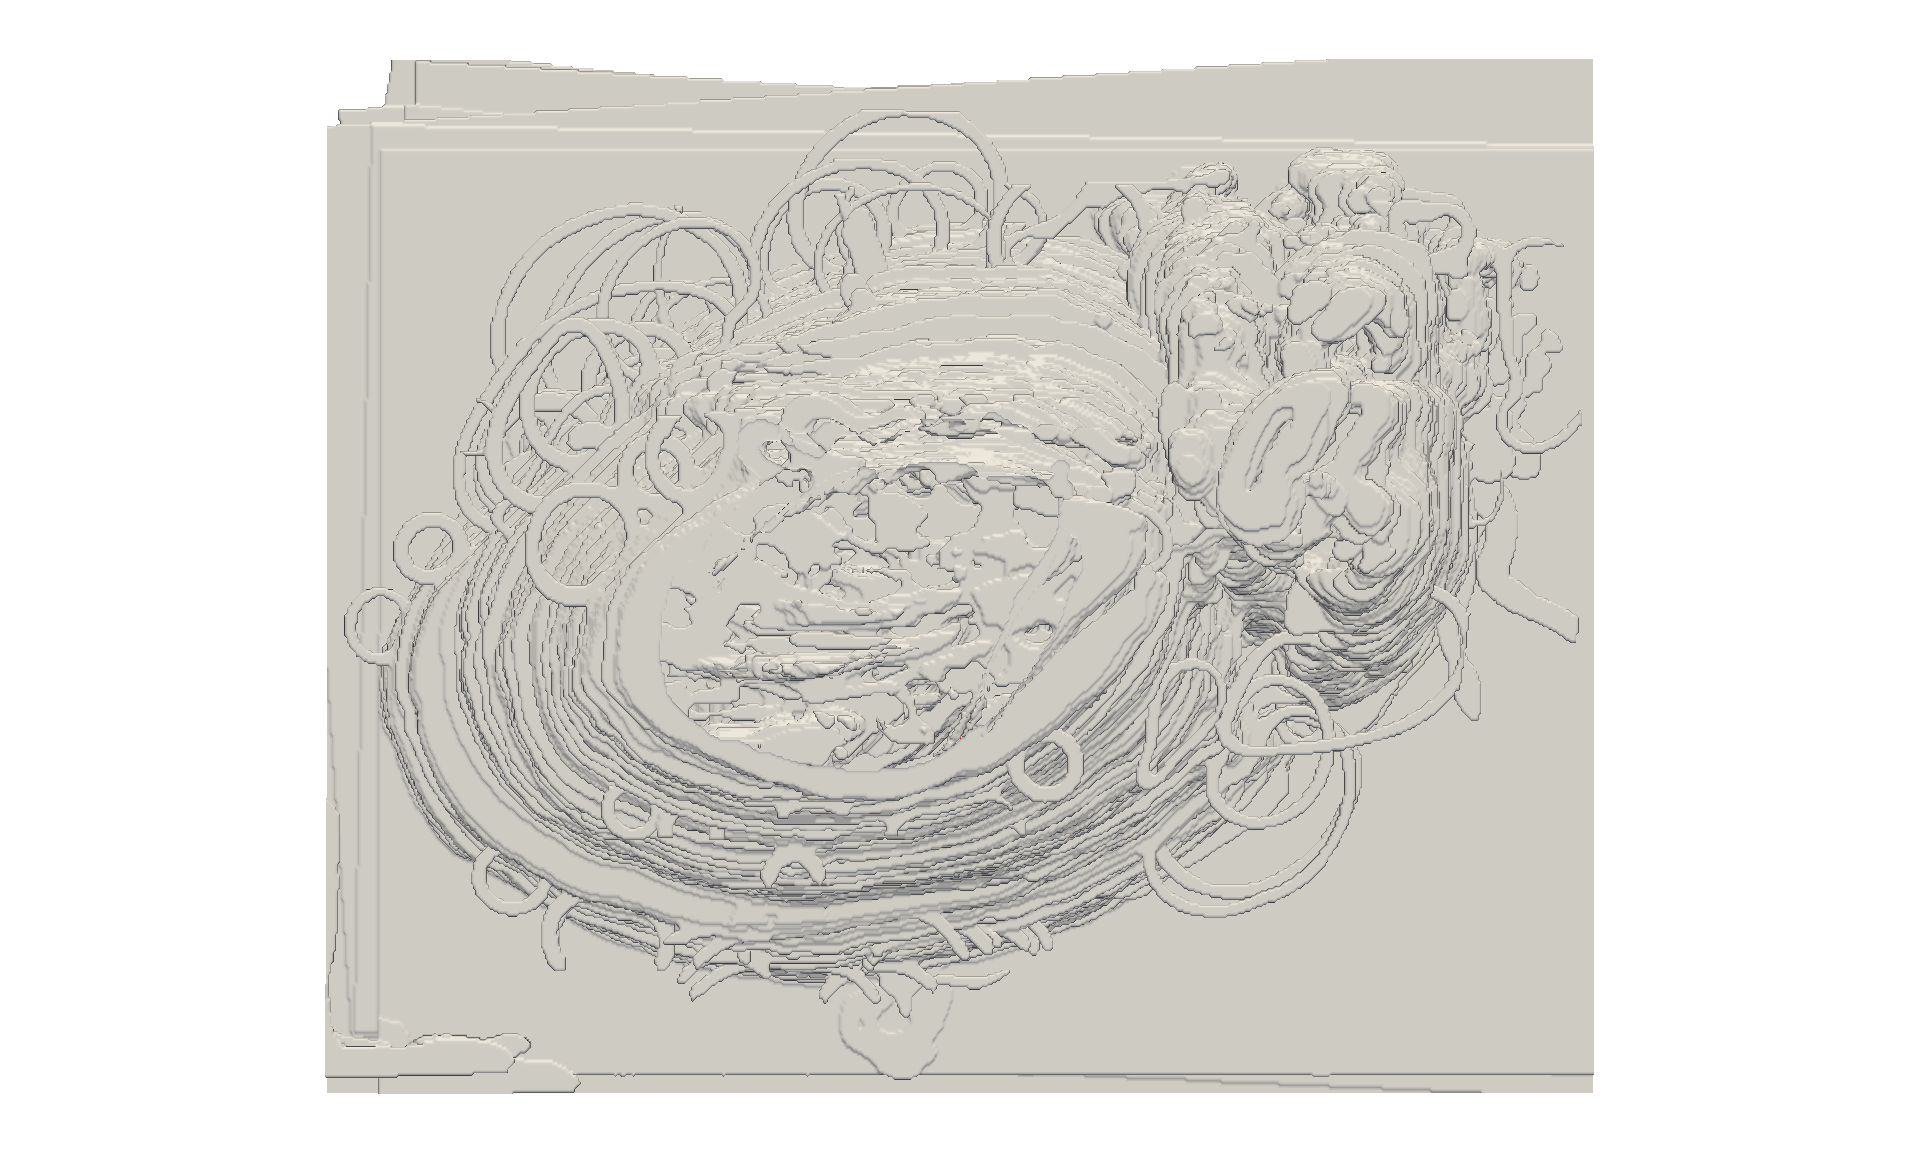
\includegraphics[width=0.9\textheight]{Ch6/Figs/Rat28/contours/whole_positive_z_affine}
	  \caption{Affine slice volume, viewed along the positive z direction.}
	  \label{fig:positive_z_affine_contour}
	\end{sidewaysfigure}
	
	Threshold segmentation contours illustrate further in Figures~\labelcref{fig:positive_x_geometric_contour,fig:negative_x_geometric_contour,fig:positive_y_geometric_contour,fig:positive_z_geometric_contour,fig:positive_x_rigid_contour,fig:negative_x_rigid_contour,fig:positive_y_rigid_contour,fig:positive_z_rigid_contour,fig:positive_x_similarity_contour,fig:negative_x_similarity_contour,fig:positive_y_similarity_contour,fig:positive_z_similarity_contour,fig:positive_x_affine_contour,fig:negative_x_affine_contour,fig:positive_y_affine_contour,fig:positive_z_affine_contour}. In all cases, contours were generated from a threshold segmentation with intensity limits 0 to 240, using the original slice images, Gaussian smoothed by a kernel of standard deviation 64, because the detail from a simple threshold on nonsmoothed images generated egregiously convoluted surfaces. Because this smoothing only operates within the plane of the slices, individual displacements between edges of adjacent slices is still clearly visible. After segmentation, a label map filter was applied to remove all but the largest connected component. This went some way to removing bubbles and other artefacts obscuring the surface of the heart. In Figures~\labelcref{fig:positive_x_geometric_contour,fig:negative_x_geometric_contour,fig:positive_y_geometric_contour,fig:positive_z_geometric_contour}, the y-dimension of the geometry bounding box is extended from 575 to 700 to encompass the increased spread of the slices. The improvements from each stage are most perceptible here, with the smoothest and most coherent surfaces in Figures~\labelcref{fig:positive_x_affine_contour,fig:negative_x_affine_contour,fig:positive_y_affine_contour,fig:positive_z_affine_contour}.
	
% section results (end)

\section{Discussion} % (fold)
\label{sec:discussion}
  We have constructed a comprehensive, generic and flexible pipeline to register histological slices to block face images, that can be configured to generate rapid results on the broadest spectrum of computational facilities, from laptop, to cluster, to shared memory supercomputer. We have developed a suite of tools to interrogate and visualise the registration process, which provides crucial insight into the tuning of parameters unavailable by any other means. A high resolution rat heart volume has been reconstructed, with coherence approximating the tissue microstructure. With recent advances in the field of histological image acquisition, and with datasets of higher and higher quality, a simple application of this pipeline will lead to even better results.
	
	An effort to apply coarse and fine grained B-spline registrations to the dataset was made. It was found that in certain regions, no matter how the system was parameterised, deformations would vary wildly from what was reasonable or physical, let alone precise. In future, it might be worthwhile to introduce constraints analogous to the physical forces and relaxations that lead to the deformations in the first place. A rudimentary framework for partial differential equations exists in ITK, and if images could be segmented to identify tissue, and physical properties such as elasticity could introduce strain terms into the cost function being optimised, results could perhaps be refined. However, the implementation would be a large undertaking, and so for the purposes of this thesis we proposed that in smaller regions, the deformations are quasi-linear, much as they are in a Reimannian manifold. This being the case, tools were developed to perform regional refined registrations with the same affine transforms, initialised by the results of full heart registrations, and these tools will be put to use in Chapter~\ref{cha:diffusion_smoothing_registration_of_high_resolution_rat_histology}.
    
  It has not escaped us that the method for choosing the various components and optimising their registration parameters is a crude and intuitive version of the optimisation algorithms applied to the image registrations. If one were to attempt to automate some of this process, at least partially, it would not easily be possible to calculate the gradient of a final in parameter space. One could perhaps develop an algorithm to perturb coordinates along the basis axes, such as the parameter scaling, the choice of metric or optimiser, the gradient descent learning rate, the regular step gradient descent relaxation factor, whether to prenormalise images etc. Two salient strategies present themselves: to split the space hierarchically into two groups of `preferred' axes, and secondary axes, then perform a prototype parameter explorative search in the preferred subspace, and for each preferred coordinate perform a cheaper, iterative optimisation in the secondary space. Alternatively, one could simply perform an iterative stochastic search across the whole space. The feasibility of this approach is unclear. In particular, the `quality' measure to be optimised is somewhat subjective, based on the goals and requirements of the scientist, and requiring detailed examination of the final volumes.
  
  Some approaches relinquished for this dataset may yield much better results in other contexts. For example, when histogram matching was tested on this dataset, there was no monotonic mapping between the intensity in the block face and that of the histology, with tissue and with non-tissue. With mutual information, a mapping need not be monotonic, but must only be one-to-one. In fact, this constraint did not hold either, since many regions of tissue in the block face images occupy the same intensity range as non-tissue.
	
	Whilst much progress has been made with traditional registration techniques in this chapter, the final volumes are still jagged and noisy. This approach is essentially a series of independent two-dimensional registrations; information flow is restricted to the two dimensions within the plane of the images, with no use of or reference to the neighbouring slices to strengthen and refine the results. In the next chapter, a new algorithm is developed, particular to this method of image acquisition, that registers adjacent slices together and uses the results of these registrations to `diffuse' each slice toward its neighbours.

% section discussion (end)

% chapter coregistration_of_high_resolution_rat_histology (end)
